\chapter{强化学习的神经科学} \label{chap:chap12}


神经科学是对神经系统的多学科研究:它们如何调节身体功能;控制行为;随着时间的推移,由于发展、学习和衰老而发生的变化;以及细胞和分子机制如何使这些功能成为可能。
强化学习最令人兴奋的方面之一是来自神经科学的越来越多的证据,证明人类和许多其他动物的神经系统实现的算法与强化学习算法惊人地对应。
本章的主要目的是解释这些相似之处,以及它们对动物奖励相关学习的神经基础的建议。


强化学习和神经科学之间最显著的联系点涉及多巴胺,这是一种深入参与哺乳动物大脑奖励处理的化学物质。
多巴胺似乎会将\textit{时间差分}误差传递给进行学习和决策的大脑结构。
\textit{多巴胺神经元活动的奖赏预测误差假说}表达了这种平行性,该假说是由计算强化学习和神经科学实验结果的汇聚引起的。
在本章中,我们讨论了这一假设,导致这一假设的神经科学发现,以及为什么它对理解大脑奖励系统有重要贡献。
我们还讨论了强化学习和神经科学之间的相似之处,这些相似之处不如\textit{多巴胺}/\textit{时间差分误差}的相似之处引人注目,但为思考动物基于回报的学习提供了有用的概念工具。
强化学习的其他元素有可能影响神经系统的研究,但它们与神经科学的联系仍相对未开发。
我们讨论了其中几个不断发展的联系,我们认为这些联系将随着时间的推移而变得越来越重要。


正如强化学习的早期历史所概述的,强化学习的许多方面都受到了神经科学的影响。
本章的第二个目标是让读者了解对我们贡献的强化学习方法关于大脑功能的想法。
从大脑功能的理论来看,强化学习的一些元素更容易理解。
\textit{资格迹}是强化学习的基本机制之一,它起源于突触的一种推测性质,突触是神经细胞(神经元)相互交流的结构。


在本章中,我们没有深入研究动物基于奖励的学习背后的神经系统的巨大复杂性:本章太短,我们不是神经科学家。
我们没有试图描述,甚至没有命名,许多大脑结构和通路,或任何分子机制,被认为与这些过程有关。
我们也没有公正地对待那些与强化学习非常一致的假设和模型的替代品。
该领域的专家之间存在分歧并不奇怪。
我们只能一窥这个引人入胜、不断发展的故事。
不过,我们希望本章能让你相信,一个非常富有成效的渠道已经出现,它将强化学习及其理论基础与动物基于奖励的学习的神经科学联系起来。


许多优秀的出版物涵盖了强化学习和神经科学之间的联系,其中一些我们在本章的最后一节中引用。
我们的处理与大多数处理不同,因为我们假设熟悉强化学习,但我们不假设了解神经科学。
我们首先简要介绍神经科学的概念,这些概念对于基本理解接下来的内容是必要的。



\section{神经科学基础} \label{sec:neuroscience_basics}

一些关于神经系统的基本信息有助于我们理解本章的内容。
我们后面提到的术语都是斜体字。
如果你已经掌握了神经科学的基本知识,跳过这一节就不会有问题。


\textit{神经元}是神经系统的主要组成部分,是专门利用电信号和化学信号处理和传递信息的细胞。
它们有多种形式,但神经元通常有一个细胞体、\textit{树突}和一个\textit{轴突}。
树突是从细胞体分支以接收来自其他神经元的输入(或者在感觉神经元的情况下也接收外部信号)的结构。
神经元的轴突是将神经元的输出传递给其他神经元(或肌肉或腺体)的纤维。
神经元的输出由一系列称为\textit{动作电位}的电脉冲组成,这些电脉冲沿着轴突传播。
动作电位也被称为\textit{脉冲},据说神经元在产生脉冲时会重新启动。
在神经网络模型中,通常使用实数来表示神经元的\textit{激活率},即某个单位时间内脉冲的平均数量。


神经元的轴突可以广泛分支,从而使神经元的动作电位达到许多目标。
神经元轴突的分支结构称为神经元轴突轴。
因为动作电位的传导是一个活跃的过程,与保险丝的燃烧没有什么不同,当动作电位到达轴突分支点时,它会“点亮”所有传出分支上的动作电位(尽管传播到分支有时会失败)。
因此,具有大轴突轴的神经元的活动可以影响许多靶位点。


\textit{突触}是一种通常位于轴突分支末端的结构,它介导一个神经元与另一个神经元的通信。
突触将信息从突触前神经元的轴突传递到突触后神经元的树突或细胞体。
除了少数例外,突触在突触前神经元的动作电位到达时会释放一种化学\textit{神经递质}。
(神经元之间直接电耦合的情况除外,但这里我们不关心这些。)
从突触突触前侧释放的神经递质分子扩散穿过突触间隙,即突触前末端和突触后神经元之间的非常小的空间,然后与突触后神经元表面的受体结合,以刺激或抑制其刺突生成活动,或以其他方式调节其行为。
一种特定的神经递质可能与几种不同类型的受体结合,每种受体对突触后神经元产生不同的影响。
例如,神经递质多巴胺至少有五种不同的受体类型可以影响突触后神经元。
许多不同的化学物质已被确定为动物神经系统中的神经递质。


当神经元似乎不受与实验者感兴趣的任务相关的突触输入的驱动时,例如,当神经元的活动与作为实验的一部分传递给受试者的刺激不相关时,神经元的背景活动是其活动水平,通常是其环速。
由于来自更宽网络的输入,或者由于神经元或其突触内的噪声,背景活动可能是不规则的。
有时,背景活动是神经元固有的动态过程的结果。
与背景活动相比,神经元的阶段性活动由通常由突触输入引起的脉冲活动爆发组成。
缓慢且经常以分级方式变化的活动,无论是否作为背景活动,都被称为神经元的\textit{强直性}活动。


突触释放的神经递质影响突触后神经元的强度或有效性是突触的有效性。
神经系统可以通过经验改变的一种方式是通过突触前和突触后神经元活动组合引起的突触能力的改变,有时还通过神经调节剂的存在,神经调节剂是一种具有除直接快速兴奋或抑制之外或除直接快速激励或抑制之外的作用的神经递质。


大脑包含几个不同的神经调控系统,由具有广泛分支轴突轴的神经元簇组成,每个系统使用不同的神经递质。
神经调控可以改变神经回路的功能,介导动机、唤醒、注意力、记忆、情绪、情绪、睡眠和体温。
重要的是,神经调节系统可以分布标量信号,如强化信号,以改变对学习至关重要的广泛分布部位突触的操作。


突触效应改变的能力称为\textit{突触可塑性}。
它是负责学习的主要机制之一。
通过学习算法调整的参数或权重对应于突触。
正如我们下面详细介绍的那样,通过神经调节剂多巴胺调节突触可塑性是大脑如何实现本书中描述的许多学习算法的一种合理机制。


\section{奖励信号、强化信号、值和预测误差} \label{sec:reward_signals}

神经科学和计算强化学习之间的联系始于大脑中的信号与在强化学习理论和算法中发挥重要作用的信号之间的相似之处。
在有限马尔可夫决策过程中,任何学习目标导向行为的问题都可以归结为代表行动、状态和奖励的三个信号。
然而,为了解释神经科学和强化学习之间的联系,我们必须不那么抽象,而是考虑在某些方面与大脑中的信号相对应的其他强化学习信号。
除了奖励信号之外,这些信号还包括强化信号(我们认为这与奖励信号不同)、价值信号和传达预测误差的信号。
当我们以这种方式通过信号的函数来标记信号时,我们是在强化学习理论的背景下进行的,在该理论中,信号对应于方程或算法中的一个项。
另一方面,当我们提到大脑中的信号时,我们指的是一种生理事件,如动作电位的爆发或神经递质的分泌。
用神经信号的功能来标记神经信号,例如将多巴胺神经元的阶段性活动称为强化信号,意味着神经信号的行为类似于相应的理论信号,并被推测为其功能类似。



揭示这些对应关系的证据涉及许多挑战。
与奖励处理相关的神经活动几乎可以在大脑的每一个部位找到,并且很难明确地解释结果,因为不同的奖励相关信号的表示往往彼此高度相关。
实验需要仔细设计,以允许一种类型的奖励相关信号以任何程度的确定性与其他信号或与奖励处理无关的大量其他信号区分开来。
尽管存在这些分歧,但已经进行了许多实验,目的是将强化学习理论和算法的各个方面与神经信号相协调,并建立了一些令人信服的联系。
为了准备研究这些链接,在本节的其余部分中,我们提醒读者根据强化学习理论,各种与奖励相关的信号意味着什么。


在上一章末尾的术语评论中,我们说过 $ R_t $ 就像动物大脑中的奖励信号,而不是动物环境中的物体或事件。
在强化学习中,奖励信号(以及智能体的环境)定义了强化学习智能体试图解决的问题。
从这方面来说,$ R_t $ 就像动物大脑中的信号,将主要奖励分配到整个大脑的各个部位。
但动物大脑中不太可能存在像 $ R_t $ 这样单一的主奖励信号。
最好将 $ R_t $ 视为一个抽象概念,它总结了大脑中许多系统生成的大量神经信号的总体影响,这些系统评估感觉和状态的奖励或惩罚质量。


强化学习中的\textit{强化信号}与奖励信号不同。
强化信号的功能是指导学习算法在智能体的策略、价值估计或环境模型中做出的改变。
例如,对于时间差分方法,时间 $ t $ 时的强化信号是时间差分误差 $ \delta_{t-1} = R_t + \gamma V(S_t) - V(S_{t-1})$。
某些算法的强化信号可能只是奖励信号,但对于大多数算法,我们认为强化信号是通过其他信息调整的奖励信号,例如 时间差分误差中的值估计。


状态值或动作值(即 $ V $ 或 $ Q $)的估计指定从长远来看对智能体来说是好是坏。
它们是对智能体未来预期累积的总奖励的预测。
智能体通过选择导致具有最大估计状态值的状态的动作,或者通过选择具有最大估计动作值的动作来做出好的决策。


预测误差衡量预期信号或感觉与实际信号或感觉之间的差异。
\textit{奖励预测误差}专门衡量预期和收到的奖励信号之间的差异,当奖励信号大于预期时为正,否则为负。 
时间差分误差是特殊类型的\textit{奖励预测误差},它表明当前和早期的长期奖励预期之间存在差异。
当神经科学家提到\textit{奖励预测误差}时,他们通常(尽管并非总是)指的是时间差分 \textit{奖励预测误差},我们在本章中简称为时间差分误差。
同样在本章中,时间差分误差通常是不依赖于动作的误差,这与 Sarsa 和 Q-学习等算法在学习动作值时使用的时间差分误差相反。
这是因为最著名的神经科学链接是用无动作时间差分误差来表述的,但我们并不意味着排除涉及依赖动作的时间差分误差的可能的类似链接。
(时间差分误差对于预测奖励以外的信号也很有用,但我们在这里不关心这种情况\cite{modayil2014prediction}。)


人们可以就神经科学数据和这些理论上定义的信号之间的联系提出许多问题。
观察到的信号是否更像是奖励信号、价值信号、预测误差、强化信号,还是完全不同的东西?
如果它是一个误差信号,它是奖励预测误差、时间差分误差还是像\textit{雷斯科拉-瓦格纳模型}误差这样的更简单的误差?
如果是时间差分误差,它是否取决于 Q-学习或 Sarsa 的 时间差分误差之类的操作?
如上所述,探测大脑来回答此类问题是极其困难的。
但实验证据表明,一种神经递质,特别是神经递质多巴胺,向奖励预测误差发出信号,并且进一步,产生多巴胺的神经元的阶段性活动实际上传达了时间差分误差(有关阶段性活动的定义,请参见第~\ref{sec:neuroscience_basics}~节)。
这一证据导致了\textit{多巴胺神经元活动的奖励预测误差假设},我们接下来将对此进行描述。


\section{奖励预测误差假设}

多巴胺神经元活动的奖励预测误差假说提出,哺乳动物中产生多巴胺的神经元的阶段性活动的功能之一是将预期未来奖励的旧估计和新估计之间的误差传递给整个大脑的目标区域。
Montague\cite{montague1996framework}首先明确提出了这一假设(尽管没有用这些确切的措辞),他们展示了强化学习中的时间差分误差概念如何解释哺乳动物多巴胺神经元阶段性活动的许多特征。
得出这一假设的实验是在 20 世纪 80 年代和 90 年代初在神经科学家\textit{沃尔夫勒姆$\cdot$舒尔茨}的实验室进行的。
第~\ref{sec:experimental_support}~节描述了这些有影响力的实验,第~\ref{sec:td_dopamine}~节解释了这些实验的结果如何与时间差分误差保持一致,本章末尾的参考文献和历史评论部分包括围绕这一有影响力的假设的发展的文献指南。


Montague\cite{montague1996framework}等人将经典条件反射的时间差分模型的时间差分误差与经典条件反射实验中产生多巴胺的神经元的相位活动进行了比较。
回想一下~\ref{sec:classical_conditioning}~节,经典调节的时间差分模型基本上是具有线性函数近似的半梯度下降 TD($ \lambda $) 算法。
Montague等人做出了几个假设来进行这种比较。
首先,由于时间差分误差可以是负的,但神经元不能有负的激活率,他们假设多巴胺神经元活动对应的量是 $ \delta_{t-1} + b_t $,其中$ b_t $是神经元的背景激活率。
负时间差分误差对应于多巴胺神经元的激活率下降到其背景速率以下。



需要第二个假设,关于每个经典条件反射试验中访问的状态以及它们如何表示为学习算法的输入。
这与我们在~\ref{sec:td_simulation}~节中针对时间差分模型讨论的问题相同。 
Montague等人选择了\textit{全串行复合}表示,如图~\ref{fig:11_1}~左栏所示,但短期内部信号序列持续到\textit{非条件刺激}开始,这里是非零奖励信号的到来。
这种表示允许时间差分误差模拟这样一个事实:多巴胺神经元活动不仅预测未来的奖励,而且对奖励预计到达的预测提示之后的时间也很敏感。
必须有某种方法来跟踪感官提示和奖励到来之间的时间。
如果刺激启动一系列内部信号,并在刺激结束后继续,并且如果刺激后的每个时间步都有不同的信号,则刺激后的每个时间步都由不同的状态表示。
因此,时间差分误差与状态相关,可能对试验中事件的时间安排很敏感。


在使用有关背景激活率和输入表示的这些假设的模拟试验中,时间差分模型的时间差分误差与多巴胺神经元相位活动非常相似。
预览我们在下面第~\ref{sec:experimental_support}~节中对这些相似性的详细描述,时间差分误差与多巴胺神经元活动的以下特征相似:
1)多巴胺神经元的阶段性反应仅在奖励事件不可预测时发生;
2)在学习早期,奖励之前的中性线索不会引起实质性的阶段性多巴胺反应,但随着学习的继续,这些线索获得预测价值并引发阶段性多巴胺反应;
3)如果更早的提示可靠地先于已经获得预测值的提示,则阶段性多巴胺反应会转移到较早的提示,而停止等待较晚的提示;
3)如果在学习之后,预测的奖励事件被忽略,多巴胺神经元的反应在奖励事件的预期时间之后不久就会降低到其基线水平以下。


尽管\textit{舒尔茨}及其同事的实验中监测到的每个多巴胺神经元并非都以所有这些方式表现,但大多数监测神经元的活动与时间差分误差之间的惊人对应关系为奖励预测误差假说提供了强有力的支持。
然而,在某些情况下,基于假设的预测与实验中观察到的结果并不相符。
输入表示的选择对于时间差分误差与多巴胺神经元活动的一些细节的匹配程度至关重要,特别是有关多巴胺神经元响应时间的细节。
关于时间差分学习的输入表示和其他特征,人们提出了不同的想法,其中一些我们在下面讨论,以使时间差分误差更好地处理数据,尽管主要的相似之处与 Montague 等人用过的\textit{全串行复合}表示相似。
总体而言,奖励预测误差假说已得到研究基于奖励的学习的神经科学家的广泛接受,并且事实证明,面对神经科学实验不断积累的结果,它具有显着的弹性。


为了准备我们对支持奖励预测误差假说的神经科学实验的描述,并提供一些背景以便可以理解该假说的重要性,我们接下来介绍一些关于多巴胺的已知知识,以及它影响的大脑结构,以及它如何参与基于奖励的学习。


\section{多巴胺} \label{sec:dopamine}

多巴胺作为神经递质由神经元产生,其细胞体主要位于哺乳动物中脑的两个神经元簇:\textit{黑质致密部}和\textit{腹侧被盖区}。
多巴胺在哺乳动物大脑的许多过程中发挥着重要作用。
其中最突出的是动机、学习、行为选择、大多数形式的成瘾以及精神分裂症和帕金森病。
多巴胺被称为神经调节剂,因为它除了直接快速兴奋或抑制目标神经元之外还执行许多功能。
尽管关于多巴胺的功能及其细胞效应的细节仍有很多未知之处,但很明显,它对于哺乳动物大脑中的奖励处理至关重要。
多巴胺并不是唯一参与奖励处理的神经调节剂,它在厌恶情况(惩罚)中的作用仍然存在争议。
多巴胺在非哺乳动物中也可以发挥不同的作用。
但没有人怀疑多巴胺对于哺乳动物(包括人类)的奖励相关过程至关重要。


早期的传统观点认为,多巴胺神经元向与学习和动机有关的多个大脑区域广播奖励信号。
这一观点源自 James Olds 和 Peter Milner 1954 年发表的一篇著名论文,该论文描述了电刺激对大鼠大脑某些区域的影响。
他们发现,对特定区域的电刺激在控制老鼠的行为方面起到了非常强大的奖励作用:“……通过这种奖励对动物行为的控制是极端的,可能超过以前在动物实验中使用的任何其他奖励。”\cite{olds1954positive}
后来的研究表明,刺激最有效地产生这种奖赏效应的位点会直接或间接地兴奋多巴胺通路,而这些通路通常会受到自然奖赏刺激的兴奋。
在人类受试者中也观察到了与大鼠相似的效应。
这些观察结果强烈表明多巴胺神经元活动发出奖励信号。


但是,如果奖励预测误差假设是正确的(即使它只解释了多巴胺神经元活动的某些特征)这种多巴胺神经元活动的传统观点并不完全正确:
多巴胺神经元的阶段性反应发出奖励预测误差的信号,而不是奖励本身。
用强化学习的术语来说,多巴胺神经元在时间 $ t $ 的相位响应对应于 $ \delta_{t-1} = R_t + \gamma V(S_t) - V(S_{t-1}) $,而不是 $ R_t $。


强化学习理论和算法有助于协调奖励预测误差观点与多巴胺信号奖励的传统观念。
在我们在本书中讨论的许多算法中,它起着强化信号的作用,这意味着它是学习的主要驱动力。
例如,$ \delta $是经典条件反射时间差分模型中的关键因素,是\textit{行动者-评论家}架构中的价值函数和策略的强化信号(第~\ref{sec:neural_ac}~节)。
动作依赖形式是 Q 学习和 Sarsa 的强化信号。
奖励信号 $ R_t $ 是 $ \delta_{t-1} $ 的关键组成部分,但它并不是其在这些算法中的强化效果的完全决定因素。
附加项 $ \gamma V(S_t) - V(S_{t-1}) $ 是 $ \delta_{t-1} $ 的高阶强化部分,即使奖励发生($ R_t \neq 0 $),如果奖励完全预测,时间差分误差也可以保持沉默。(在下面第~\ref{sec:td_dopamine}~节中有完整解释)。


事实上,仔细观察 Olds 和 Milner 1954 年的论文就会发现,它主要是关于电刺激在仪器调节任务中的强化作用。
电刺激不仅通过多巴胺对动机的影响激发了老鼠的行为,还使老鼠很快学会了通过按下杠杆来刺激自己,而它们会经常长时间这样做。
电刺激触发的多巴胺神经元的活动增强了大鼠的杠杆按压。


最近使用光遗传学方法的实验证实了多巴胺神经元的相位反应作为强化信号的作用。
这些方法使神经科学家能够在清醒行为动物中以毫秒为单位精确控制所选神经元类型的活动。
光遗传学方法将光敏蛋白引入选定的神经元类型中,以便可以通过激光的灰烬激活或沉默这些神经元。
第一个使用光遗传学方法研究多巴胺神经元的实验表明,在小鼠体内产生多巴胺神经元阶段性激活的光遗传学刺激足以使小鼠更喜欢接受刺激的室的一侧,而不是接受刺激的室的另一侧 无刺激或频率较低的刺激\cite{tsai2009phasic}。
在另一个例子中\cite{steinberg2013causal}使用多巴胺神经元的光遗传学激活,在预期奖励刺激的时间在大鼠中产生多巴胺神经元活动的人工爆发,但在多巴胺神经元活动正常暂停时却忽略了奖励刺激。
当这些停顿被人工爆发所取代时,当反应通常由于缺乏强化而减少时(在灭绝试验中),反应就会持续,而当反应通常由于已经预测到奖励而被阻止时,学习就会被启用(阻塞范式; 第~\ref{sec:blocking_higher_order}~节)。


多巴胺增强功能的额外证据来自于水果的光遗传学实验,但在这些动物中,多巴胺的作用与其在哺乳动物中的作用相反:光触发的多巴胺神经元活动爆发就像电击足部一样增强回避行为 ,至少对于激活的多巴胺神经元群体而言\cite{claridge2009writing}。
尽管这些光遗传学实验都没有表明相位多巴胺神经元活动特别像时间差分误差,但它们令人信服地证明了相位多巴胺神经元活动就像算法中的强化信号一样(或者可能像水果中的负行为) 用于预测(经典条件反射)和控制(仪器条件反射)。


多巴胺神经元特别适合向大脑的许多区域广播强化信号。
这些神经元具有巨大的轴突乔木,每个神经元释放的多巴胺的突触位点比典型神经元的轴突多出 100 至 1,000 倍。
图~\ref{fig:12_1}~显示了单个多巴胺神经元的轴突,其细胞体位于大鼠大脑的\textit{黑质致密部}中。
\textit{黑质致密部}或\textit{中脑腹侧被盖区}多巴胺神经元的每个轴突在目标大脑区域的神经元树突上产生大约 500,000 个突触接触。


\begin{figure}[!htb]
	\centering
	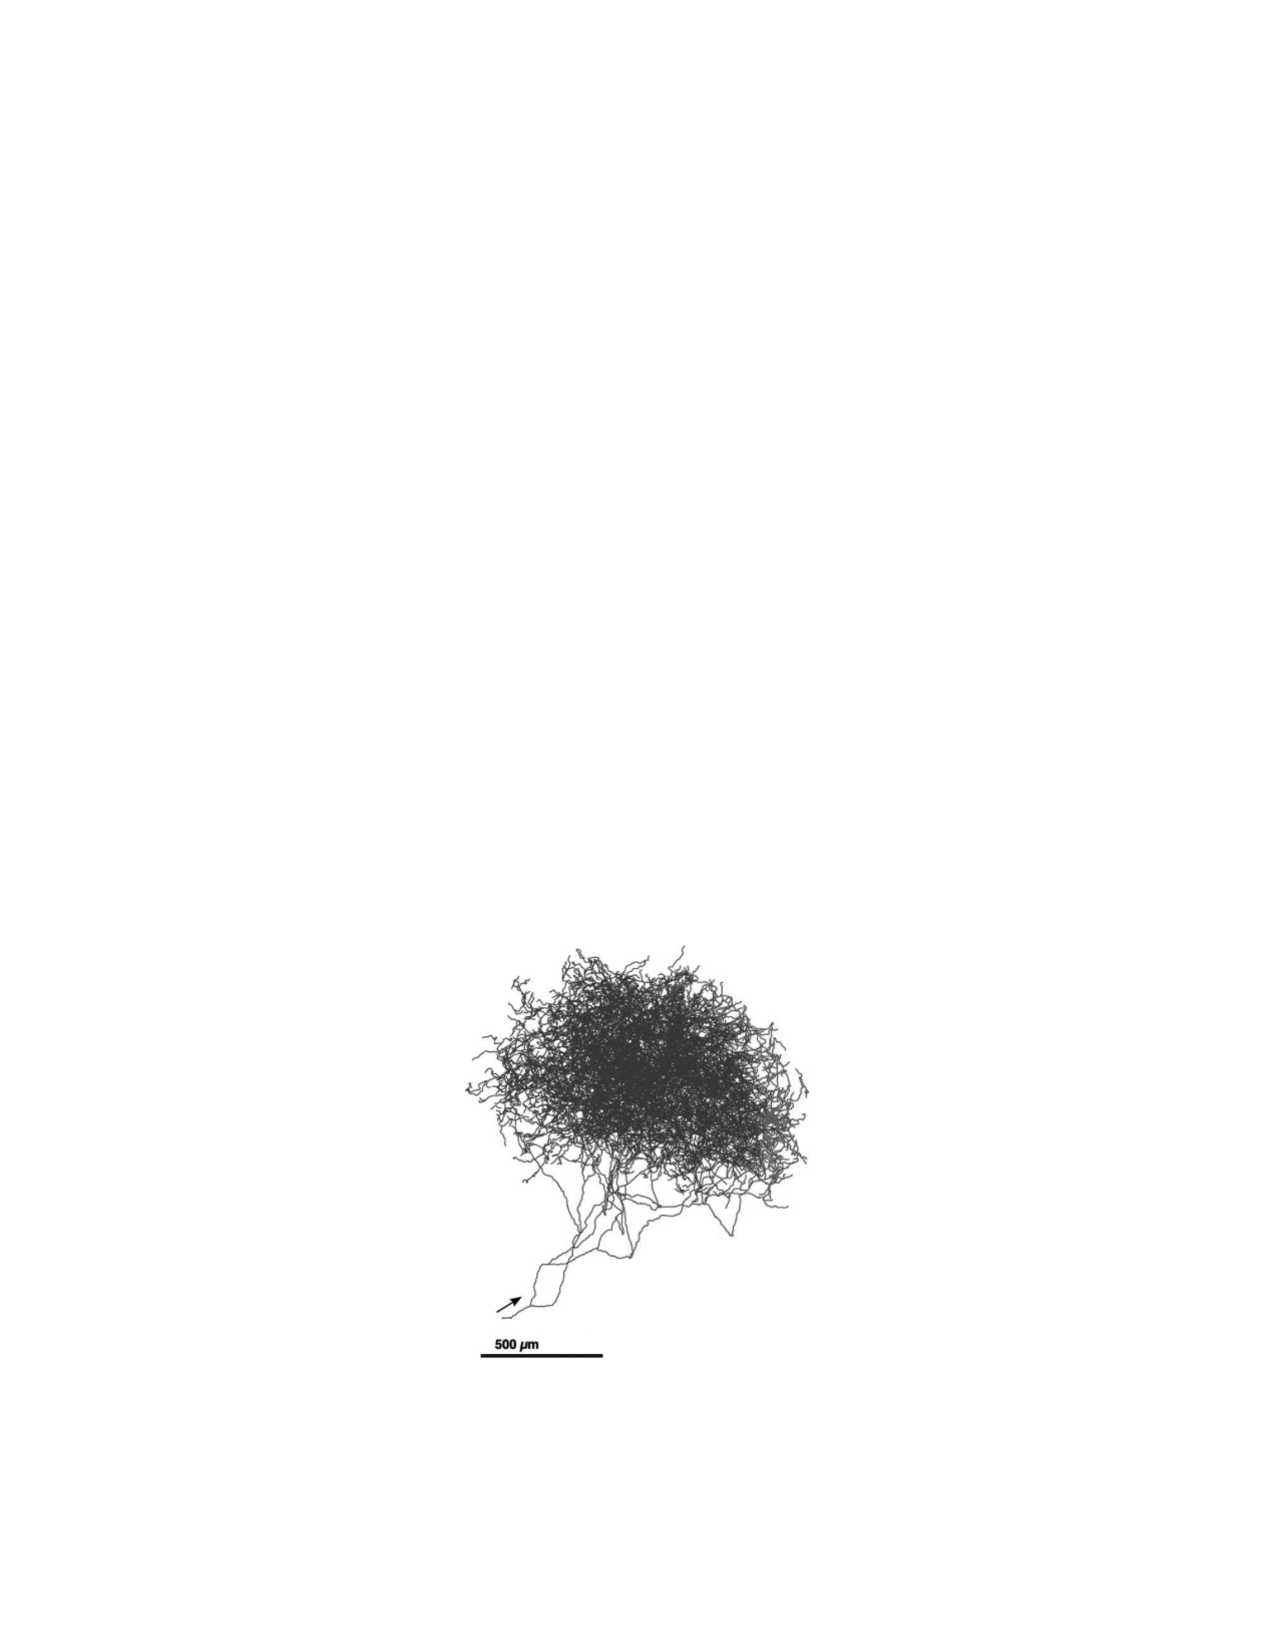
\includegraphics[width=0.5\linewidth]{chap12/fig_12_1}
	\caption{产生多巴胺作为神经递质的单个神经元的轴突乔木,其细胞体位于大鼠大脑的\textit{黑质致密部}中。
		这些轴突与目标大脑区域中的大量神经元树突进行突触接触。 \label{fig:12_1}}
\end{figure}


如果多巴胺神经元像强化学习那样广播强化信号,那么由于这是一个标量信号,即单个数字,因此\textit{黑质致密部}和\textit{中脑腹侧被盖区}中的所有多巴胺神经元将被期望或多或少相同地激活,以便它们近乎同步地行动,向轴突目标的所有部位发送相同的信号。 
尽管人们普遍认为多巴胺神经元确实像这样一起行动,但现代证据指出了更复杂的情况,即不同的多巴胺神经元亚群对输入的反应不同,具体取决于它们发送信号的结构和不同的结构。
这些信号以不同的方式作用于其目标结构。
多巴胺除了发出\textit{奖励预测误差}信号之外还有其他功能,即使对于发送\textit{奖励预测误差}信号的多巴胺神经元来说,根据这些结构在产生强化行为中所扮演的角色,将不同的\textit{奖励预测误差}发送到不同的结构也是有意义的。
这超出了我们在本书中详细讨论的范围,但从强化学习的角度来看,向量值\textit{奖励预测误差}信号是有意义的,因为决策可以分解为单独的子决策,或者更一般地说,作为解决问题的结构版本的一种方法。
信用分配问题:如何在可能参与制定决策的许多组成结构中分配决策成功的功劳(或失败的责任)?
我们在下面的~\ref{sec:collective_rl}~节中对此进行了更多讨论。


大多数多巴胺神经元的轴突与额叶皮层和基底神经节中的神经元进行突触接触,这些区域是大脑中参与随意运动、决策、学习和认知功能(例如计划)的区域。
由于大多数将多巴胺与强化学习相关的想法都集中在基底神经节上,并且多巴胺神经元的连接在那里特别密集,因此我们在这里重点关注基底神经节。
基底神经节是位于前脑底部的神经元群或细胞核的集合。 基底神经节的主要输入结构称为纹状体。
基本上所有的大脑皮层以及其他结构都向纹状体提供输入。
皮层神经元的活动传达了有关感觉输入、内部状态和运动活动的大量信息。
皮质神经元的轴突与纹状体主要输入/输出神经元的树突进行突触接触,称为中棘神经元。
纹状体的输出通过其他基底神经节核和丘脑循环回皮层的额叶区域和运动区域,使纹状体能够影响运动、抽象决策过程和奖励处理。
纹状体的两个主要细分对于强化学习很重要:背侧纹状体,主要参与影响动作选择;
腹侧纹状体,被认为对奖励处理的不同方面至关重要,包括将情感价值分配给感觉。



中型多刺神经元的树突上覆盖着刺,皮层神经元的轴突在其尖端进行突触接触。
与这些棘进行突触接触的还有多巴胺神经元的轴突(图~\ref{fig:12_2})。
这种排列汇集了皮质神经元的突触前活动、中型多棘神经元的突触后活动以及多巴胺神经元的输入。
这些刺上实际发生的事情很复杂并且尚未完全了解。
图~\ref{fig:12_2}~通过显示两种类型的多巴胺受体、谷氨酸受体(皮层输入的神经递质)以及各种信号相互作用的多种方式暗示了复杂性。
但越来越多的证据表明,从皮层到纹状体通路上的突触(神经科学家称之为皮层纹状体突触)的效率变化很大程度上取决于适当定时的多巴胺信号。



\begin{figure}[!htb]
	\centering
	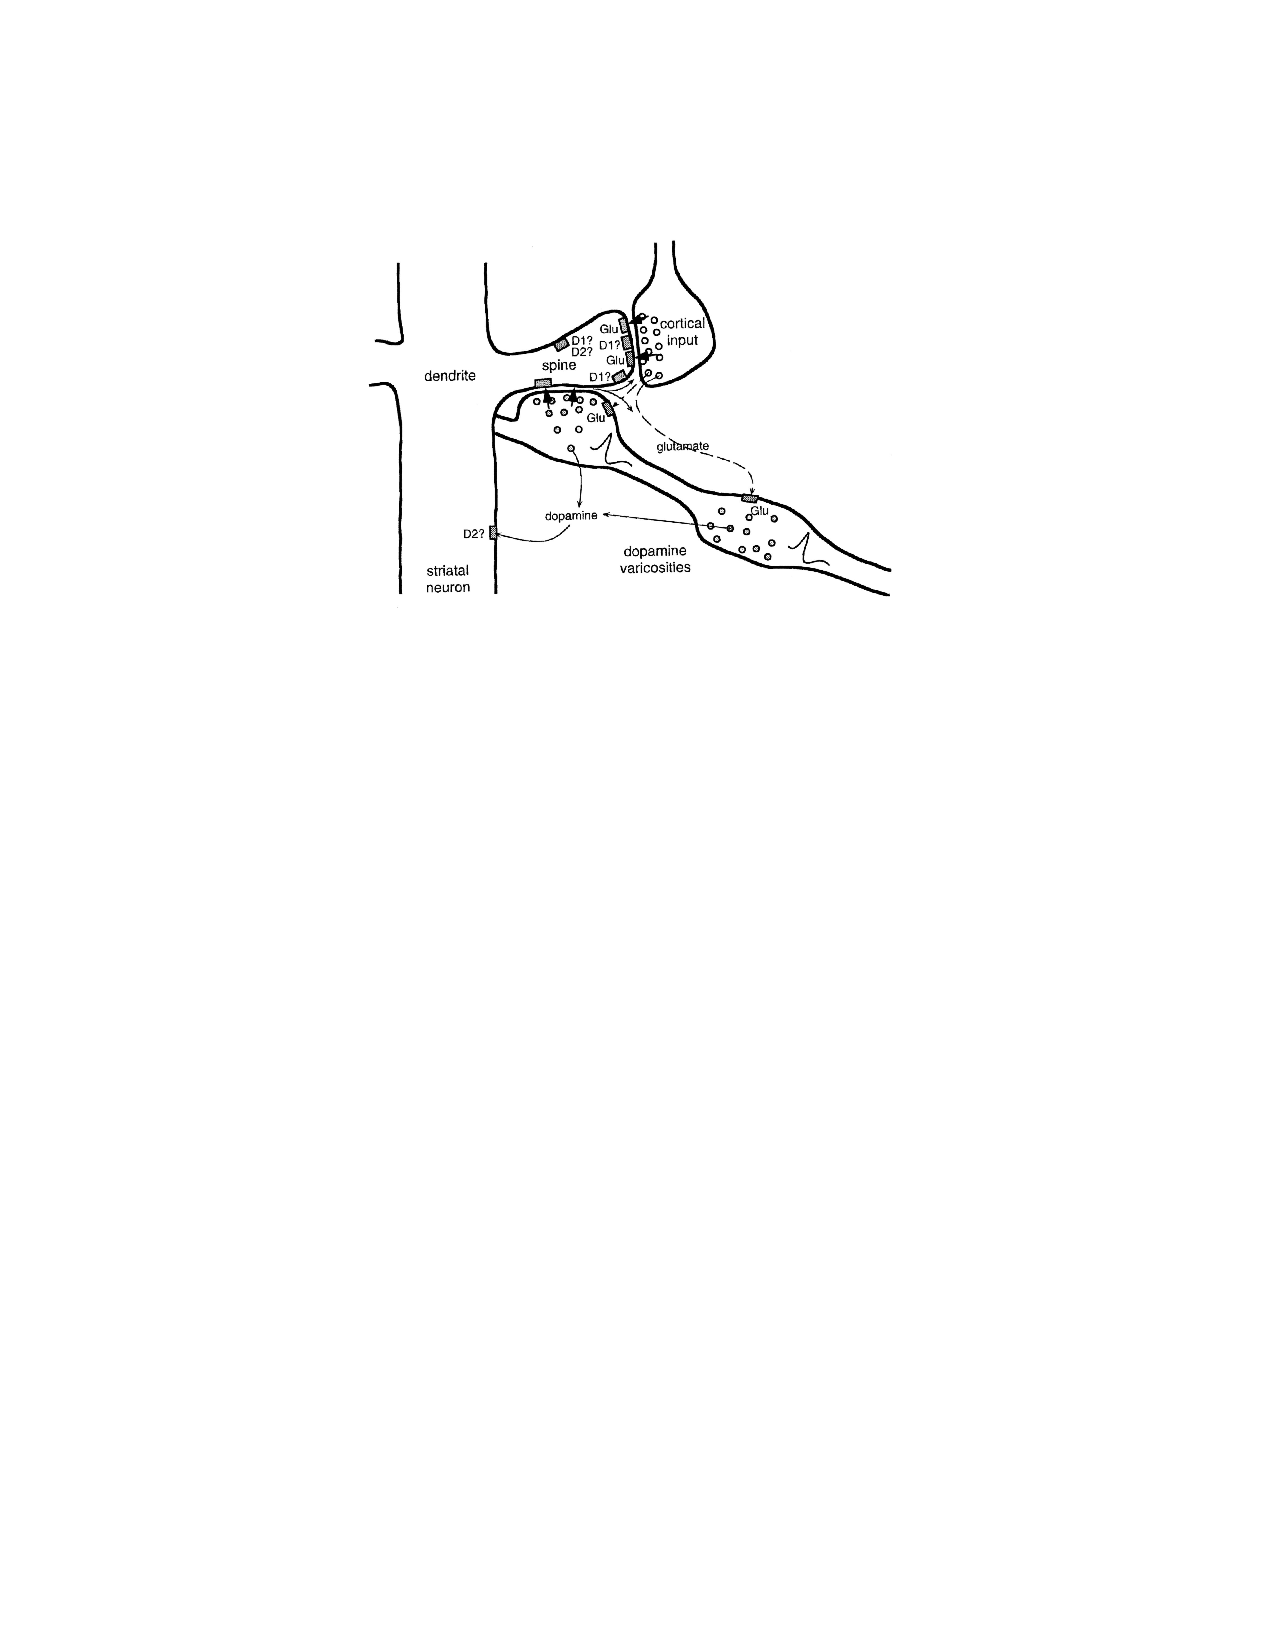
\includegraphics[width=0.7\linewidth]{chap12/fig_12_2}
	\caption{纹状体神经元的脊柱显示来自皮层和多巴胺神经元的输入。
		皮层神经元的轴突通过皮质纹状体突触影响纹状体神经元,在覆盖纹状体神经元树突的棘尖释放神经递质谷氨酸。
		显示\textit{腹侧被盖区}或\textit{黑质致密部}多巴胺神经元的轴突经过脊柱(从右下)。
		该轴突上的“多巴胺静脉曲张”在脊柱干处或附近释放多巴胺,其排列将皮质的突触前输入、纹状体神经元的突触后活动和多巴胺结合在一起,使得几种类型的学习规则控制可塑性成为可能。
		多巴胺神经元的每个轴突与大约 500,000 个棘突的茎部进行突触接触,这里通过其他神经递质途径和多种受体类型(例如多巴胺通过的 D1 和 D2 多巴胺受体)显示了我们讨论中省略的一些复杂性\cite{schultz1998predictive}。
		\label{fig:12_2}}
\end{figure}



\section{奖励预测误差假设的实验支持} \label{sec:experimental_support}

多巴胺神经元对强烈的、新颖的或意想不到的视觉和听觉刺激做出反应,这些刺激会引发眼睛和身体的运动,但它们的活动很少与运动本身相关。
这是令人惊讶的,因为多巴胺神经元的退化是帕金森病的一个原因,帕金森病的症状包括运动障碍,特别是自发运动的缺陷。
由于多巴胺神经元活动与刺激触发的眼睛和身体运动之间的微弱关系,\textit{舒尔茨}\cite{romo1990dopamine,schultz1990dopamine}通过记录猴子移动手臂时多巴胺神经元的活动和肌肉活动,朝着奖励预测误差假说迈出了第一步。


他们训练两只猴子,当猴子看到并听到箱子的门打开时,将手伸入装有一些苹果、一块饼干或葡萄干的箱子。
然后猴子就可以抓住食物并将其送到嘴里。
当猴子擅长这项工作后,它又接受了另外两项任务的训练。
第一项任务的目的是观察当自发运动时多巴胺神经元会做什么。
箱子是开着的,但从上面盖住了,这样猴子就看不到里面的东西,但可以从下面伸手进去。
没有出现任何触发刺激,在猴子伸手去拿食物并吃掉后,实验者通常(尽管并非总是如此)在猴子看不见的情况下,将食物粘在一根坚硬的金属丝上,以取代箱子中的食物。
在这里,\textit{舒尔茨}监测到的多巴胺神经元的活动与猴子的运动无关,但每当猴子第一次接触食物时,这些神经元中的很大一部分都会产生阶段性反应。
当猴子只触摸电线或在没有食物的情况下探索箱子时,这些神经元不会做出反应。
这是神经元对食物而不是任务的其他方面做出反应的有力证据。


\textit{舒尔茨}的第二个任务的目的是看看当刺激触发运动时会发生什么。
这项任务使用了一个带有可移动盖子的不同箱子。
箱子打开的景象和声音引发了向箱子伸出手的动作。
在这种情况下,\textit{舒尔茨}发现,经过一段时间的训练,多巴胺神经元不再对食物的触摸做出反应,而是对食物箱盖打开的视觉和声音做出反应。
这些神经元的阶段性反应已经从奖励本身转变为预测奖励可用性的刺激。
在后续研究中,\textit{舒尔茨}发现,他们监测的大多数多巴胺神经元的活动在行为任务背景之外对箱子打开的景象和声音没有反应。
这些观察结果表明,多巴胺神经元既不响应运动的启动,也不响应刺激的感觉特性,而是发出奖励期望的信号。


\textit{舒尔茨}的小组进行了许多涉及\textit{黑质致密部}和\textit{中脑腹侧被盖区}多巴胺神经元的其他研究。
一系列特定的实验具有重要意义,表明多巴胺神经元的相位反应对应于\textit{时间差分}误差,而不是像\textit{雷斯科拉-瓦格纳模型}(\ref{sec:instrumental_conditioning}) 中的那些更简单的误差。
在第一个实验中\cite{ljungberg1992responses},猴子被训练在灯光亮起后按下杠杆作为“触发提示”,以获得一滴苹果汁。
正如罗莫和舒尔茨之前观察到的那样,许多多巴胺神经元最初对奖励--果汁滴做出反应(图~\ref{fig:12_3},上图)。
但随着训练的继续,许多神经元失去了奖励反应,并产生了对预测奖励的光照射的反应(图~\ref{fig:12_3},中图)。
随着持续的训练,按下杠杆的速度变得更快,而对触发信号做出反应的多巴胺神经元的数量却减少了。


\begin{figure}[!htb]
	\centering
	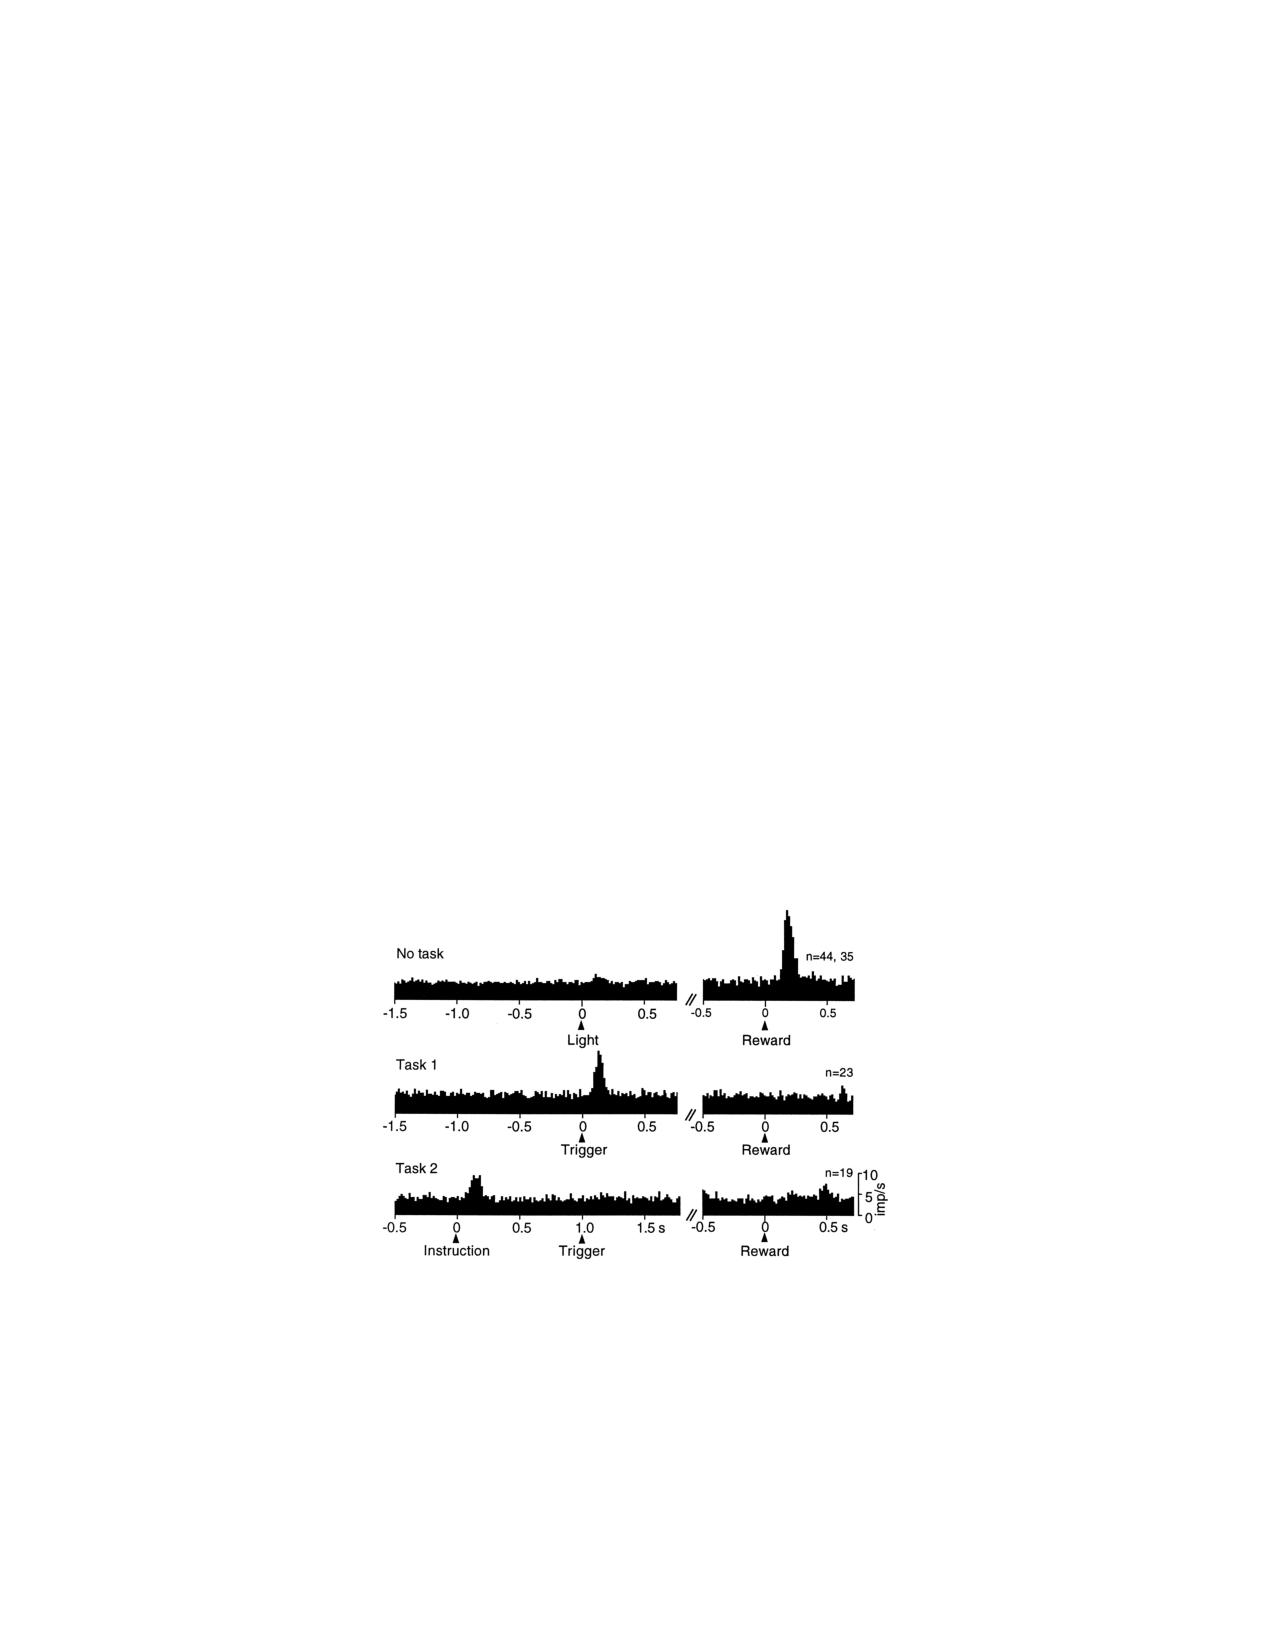
\includegraphics[width=0.55\linewidth]{chap12/fig_12_3}
	\caption{多巴胺神经元的反应从最初对初级奖励的反应转变为早期的预测刺激。
		这些是受监测的多巴胺神经元在小时间间隔内产生的动作电位数量的图,是所有受监测的多巴胺神经元(这些数据的范围从 23 到 44 个神经元)的平均值。
		上图:多巴胺神经元被意外输送的一滴苹果汁激活。
		中图:通过学习,多巴胺神经元对奖励预测触发线索产生反应,并失去对奖励传递的反应。
		下图:通过在触发提示之前添加 1 秒的指令提示,多巴胺神经元将其反应从触发提示转移到更早的指令提示\cite{schultz1994reward}。
		\label{fig:12_3}}
\end{figure}



在这项研究之后,同样的猴子接受了一项新任务的训练\cite{schultz1993responses}。
在这里,猴子面对着两个杠杆,每个杠杆上方都有一盏灯。
点亮其中一个灯是一个“指令提示”,指示两个杠杆中的哪一个会产生一滴苹果汁。
在此任务中,指令提示在前一个任务的触发提示之前有 1 秒的固定间隔。
猴子学会了在看到触发提示之前不伸手,多巴胺神经元活动增加,但现在受监测的多巴胺神经元的反应几乎完全发生在较早的指令提示上,而不是触发提示上(图~\ref{fig:12_3},底部面板)。
当任务被很好地学习时,对指令线索做出反应的多巴胺神经元的数量再次大大减少。
在学习这些任务的过程中,多巴胺神经元活动从最初对奖励的反应转变为对早期预测刺激的反应,首先发展到触发刺激,然后发展到更早的指令提示。
随着反应时间提前,它会从后来的刺激中消失。
这种对较早奖励预测变量的反应的转变,同时失去对较晚预测变量的反应是\textit{时间差分}学习的一个标志(例如,参见图~\ref{fig:12_4})。


\begin{figure}[!htb]
	\centering
	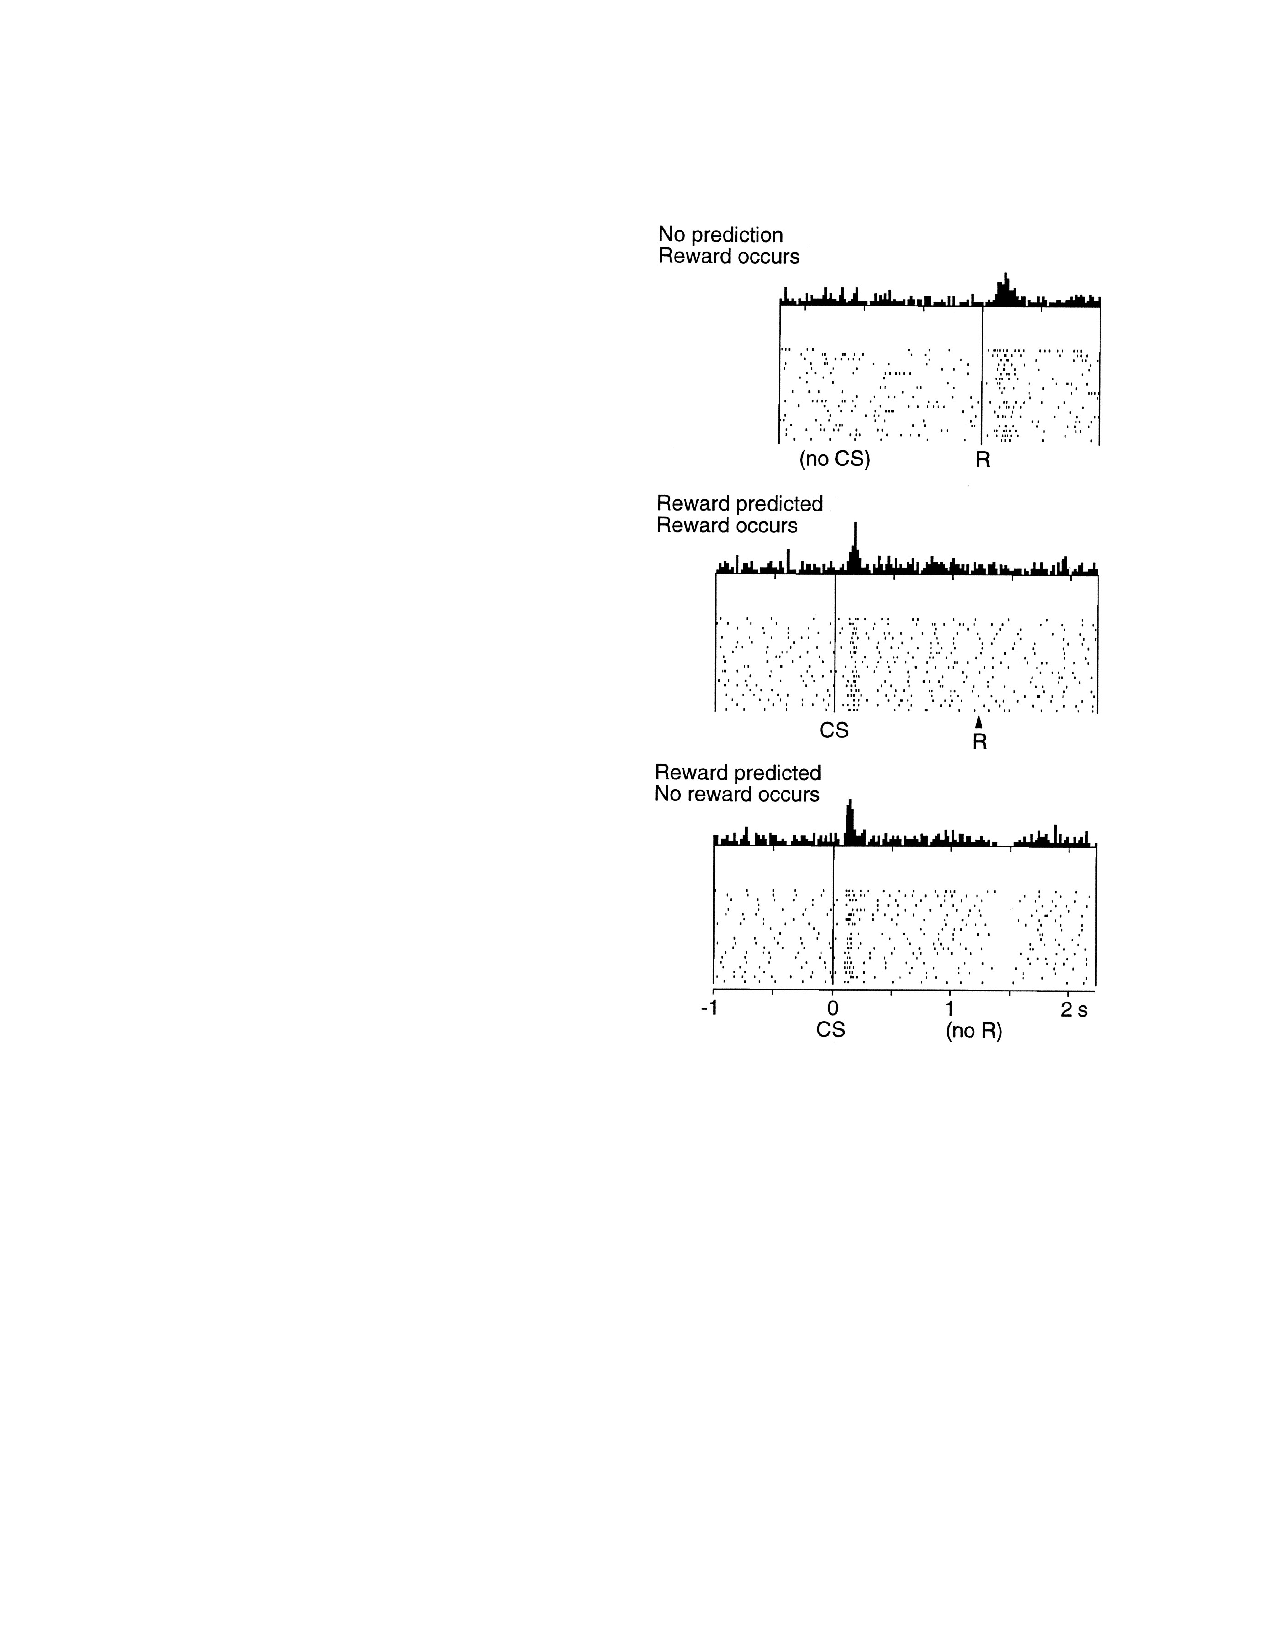
\includegraphics[width=0.45\linewidth]{chap12/fig_12_4}
	\caption{在预期奖励未能发生后不久,多巴胺神经元的反应就会降至基线以下。
		上图:一滴苹果汁的意外输送会激活多巴胺神经元。
		中:多巴胺神经元对预测奖励的\textit{条件刺激}做出反应,但不对奖励本身做出反应。
		下图:当\textit{条件刺激}预测的奖励未能发生时,多巴胺神经元的活动在预期奖励发生后不久就会降至基线以下。
		每个面板的顶部显示了受监测的多巴胺神经元在指定时间附近的小时间间隔内产生的动作电位的平均数量。
		下面的光栅图显示了受监测的单个多巴胺神经元的活动模式;
		每个点代表一个动作电位\cite{schultz1997neural}。
		\label{fig:12_4}}
\end{figure}


刚刚描述的任务揭示了多巴胺神经元活动与\textit{时间差分}学习共有的另一个特性。
猴子有时会按错键,即按指示以外的键,因此得不到任何奖励。
在这些试验中,许多多巴胺神经元在奖励的通常传递时间后不久表现出其环率急剧下降至基线以下,并且这种情况发生时没有任何外部线索来标记通常的奖励传递时间(图~\ref{fig:12_4}) 。
不知何故,猴子在内部记录了奖励的时间。
(响应时间是需要修改最简单版本的\textit{时间差分}学习的一个领域,以考虑多巴胺神经元响应时间的一些细节。
我们将在下一节中考虑这个问题。)


根据上述研究的观察结果,\textit{舒尔茨}和他的团队得出结论,多巴胺神经元对未预测的奖励和最早的奖励预测因子有反应,如果奖励或奖励预测因子没有在预期时间出现,多巴胺神经元的活动就会下降到基线以下。
熟悉强化学习的研究人员很快认识到,这些结果与\textit{时间差分}算法中\textit{时间差分}误差作为强化信号的表现惊人地相似。
下一节将通过一个具体示例详细探讨这种相似性。


\section{时间差分误差/对应的多巴胺} \label{sec:td_dopamine}

本节解释\textit{时间差分}误差与刚才描述的实验中观察到的多巴胺神经元的相位反应之间的对应关系。
我们研究了在类似上述任务的学习过程中如何变化,其中猴子首先看到指令提示,然后在固定的时间内必须正确响应触发提示才能获得奖励。
我们使用此任务的简单理想化版本,但我们比平常更详细,因为我们想强调\textit{时间差分}误差和多巴胺神经元活动之间并行的理论基础。


第一个简化假设是智能体已经学会了获得奖励所需的操作。
那么它的任务就是学习对其经历的状态序列的未来奖励的准确预测。
这是一个预测任务,或者更技术地说,是一个策略评估任务:学习固定策略的价值函数。
要学习的价值函数为每个状态分配一个值,该值预测如果智能体根据给定策略选择操作,该状态将遵循的回报,其中回报是所有未来奖励的(可能是折扣的)总和。
作为猴子情况的模型,这是不现实的,因为猴子可能会在学习正确行动的同时学习这些预测(就像学习策略和价值函数的强化学习算法一样,例如\textit{行动者}\textit{评论家}算法),但这种场景比同时学习策略和价值函数的场景更容易描述。


现在想象一下,智能体的经验分为多个试验,在每个试验中重复相同的状态序列,并且在试验期间的每个时间步上发生不同的状态。
进一步想象一下,预测的回报仅限于试验的回报,这使得试验类似于我们定义的强化学习事件。
当然,实际上,预测的回报并不局限于单次试验,试验之间的时间间隔是决定动物学到什么的重要因素。
对于时间差分学习来说也是如此,但这里我们假设回报不会通过多次试验累积。
鉴于此,\textit{舒尔茨}及其同事进行的实验相当于强化学习的一个阶段。
(尽管在本次讨论中,我们将使用术语“试验”而不是“情节”,以便更好地与实验联系起来。)


像往常一样,我们还需要对状态如何表示为学习算法的输入做出假设,该假设会影响\textit{时间差分误差}与多巴胺神经元活动的对应程度。
我们稍后讨论这个问题,但目前我们假设Montague等人使用相同的CSC表示\cite{montague1996framework}。
其中,在试验的每个时间步骤访问的每个州都有一个单独的内部刺激。
这将流程简化为本书第一部分中介绍的表格案例。
最后,我们假设智能体使用 TD(0) 来学习值函数 $V$ ,该函数存储在所有状态下初始化为零的查找表中。
我们还假设这是一项确定性任务,并且折扣因子$\gamma$ 非常接近 1,因此我们可以忽略它。


图~\ref{fig:12_5}~显示了 $R$、$V$ 和 $\delta$ 在该策略评估任务的几个学习阶段的时间过程。 
时间轴表示在试验中访问一系列状态的时间间隔(为了清楚起见,我们省略了显示各个状态)。
在每次试验中,奖励信号为零,除非智能体达到奖励状态(显示在时间线右端附近),此时奖励信号变为某个正数(例如 $R^{\star}$)。
\textit{时间差分}学习的目标是预测试验中访问的每个状态的返回,在这种未贴现的情况下,并假设预测仅限于单个试验,对于每个状态这简单地说是$R^{\star}$。


\begin{figure}[!htb]
	\centering
	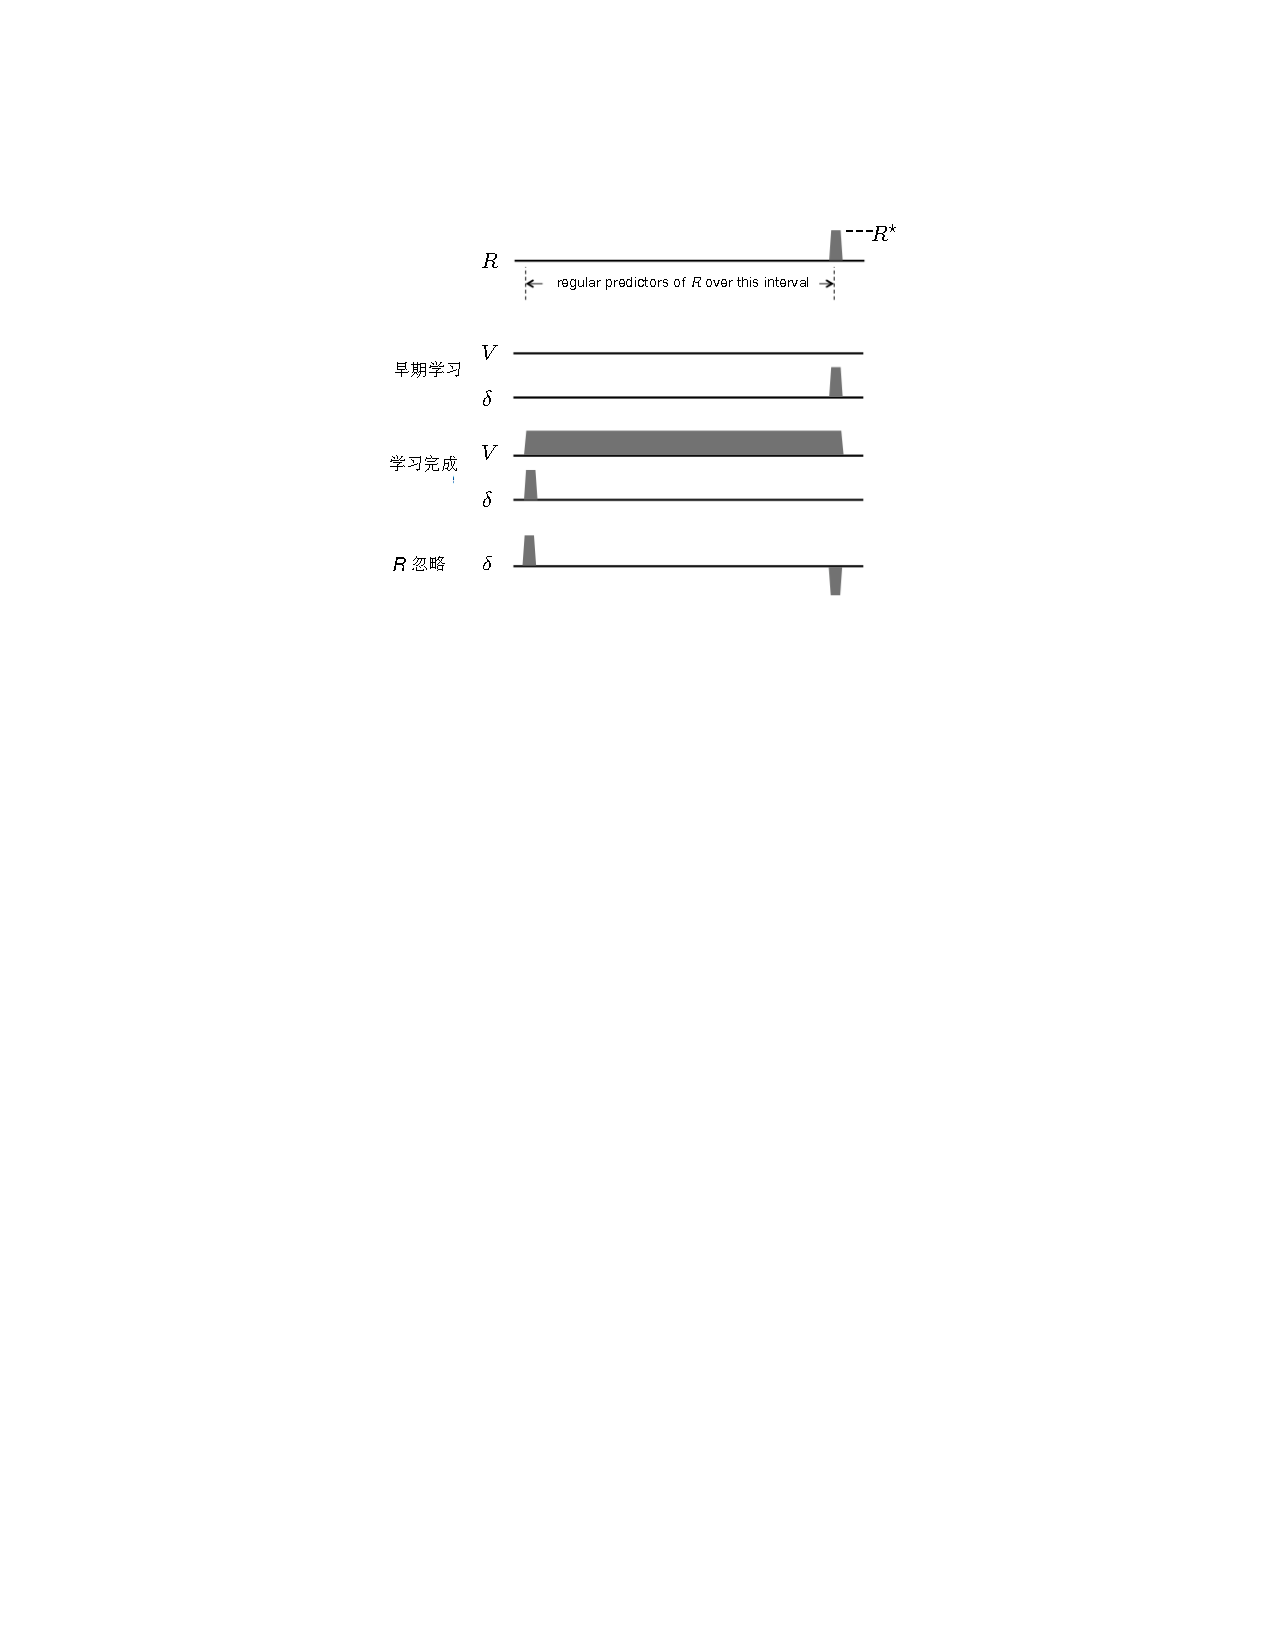
\includegraphics[width=0.5\linewidth]{chap12/fig_12_5}
	\caption{\textit{时间差分}学习过程中\textit{时间差分}误差的行为与多巴胺神经元的阶段性激活特征一致。
		(这里是时间 $t$ 时的\textit{时间差分}误差,即 $\delta_{t-1}$)。
		顶部:状态序列,显示为常规预测变量的区间,后面跟着非零奖励 $R^{\star}$。
		\textit{早期学习}:初始值函数 $V$ 和初始值,最初等于 $R^{\star}$。
		\textit{学习完成}:价值函数准确地预测了未来的奖励,在最早的预测状态下为正,在非零奖励时 $\delta = 0$。
		\textit{$R^{\star}$忽略}:当预测奖励被忽略时,变为负数。
		请参阅文本以获取发生这种情况的完整解释。
		\label{fig:12_5}}
\end{figure}


奖励状态之前是一系列奖励预测状态,最早的奖励预测状态显示在时间线左端附近。
这类似于试验开始附近的状态,例如类似于上述\textit{舒尔茨}等人\cite{schultz1993responses}的猴子实验试验中由指令提示标记的状态。
(当然,实际上,先前试验中访问的状态甚至是更早的奖励预测状态,但是因为我们将预测限制在单个试验中,所以这些状态不符合本次试验奖励的预测因子。
下面我们给出一个更令人满意的,但更多的 摘要,最早的奖励预测状态的描述。)
试验中最新的奖励预测状态是紧接在试验的奖励状态之前的状态。
这是图~\ref{fig:12_5}~中时间线最右端附近的状态。
请注意,试验的奖励状态并不能预测该试验的回报:该状态的值将预测所有以下试验的回报,在这里我们假设在这个情景公式中为零。


图~\ref{fig:12_5}~显示了 $V$ 和 $\delta$ 的首次尝试时间课程,并标记为“早期学习”。 
因为除达到奖励状态外,整个试验过程中奖励信号为零,并且所有 $V$值均为零,因此\textit{时间差分}误差也为零,直到变为 $R^{\star}$ 处于奖励状态。
这是因为 $\delta_{t-1} = R_t + V_t - V_{t+1} = R_t + 0 - 0 = R_t$,当奖励发生时,在等于 $R^{\star}$ 之前它为零。
这里$V_t$和 $V_{t-1}$ 分别是试验中在时间$t$和$t-1$访问的状态的估计值。
此学习阶段的\textit{时间差分}误差类似于多巴胺神经元在训练开始时对不可预测的奖励(例如一滴苹果汁)的反应。



在第一个试验和所有后续试验中,TD(0) 更新发生在每个状态转换处。
这会连续增加奖励预测状态的值,并且增加从奖励状态向后传播,直到值 收敛到正确的回报预测。
在这种情况下(因为我们假设没有折扣)正确的预测等于 $R^{\star}$ 对于所有奖励预测状态。
这可以在图~\ref{fig:12_5}~中看到,作为标记为“学习完成”的 $V$ 的图,其中从最早到最新的奖励预测状态的所有状态的值都等于 $R^\star$。
最早奖励预测状态之前的状态值仍然很低(图~\ref{fig:12_5}~显示为零),因为它们不是可靠的奖励预测器。


当学习完成时,即当 $V$ 达到其正确值时,与任何奖励预测状态的转换相关的\textit{时间差分}误差为零,因为预测现在是准确的。
这是因为对于从奖励预测状态到另一个奖励预测状态的转变,我们有$\delta_{t-1} = R_t + V_t - V_{t-1} = 0 + R^{\star} - R^{\star} = 0$,对于从最新奖励预测状态到奖励状态的转变,我们有 $\delta_{t-1} = R_t + V_t - V_{t-1}$。
另一方面,从任何状态转换到最早的奖励预测状态的\textit{时间差分}误差都是正的,因为该状态的低值与后续奖励预测状态的较大值之间不匹配。
事实上,如果最早奖励预测状态之前的状态值为零,那么在过渡到最早奖励预测状态之后,我们将得到 $\delta_{t-1} = R_t + V_t - V_{t-1} = 0 + R^{\star} - 0 = R^{\star}$。 
图~\ref{fig:12_5}~中的“学习完成”图显示了最早奖励预测状态下的正值,而其他地方为零。


过渡到最早的奖励预测状态时的正\textit{时间差分}误差类似于多巴胺对最早预测奖励的刺激的持续反应。
出于同样的原因,当学习完成时,从最新的奖励预测状态到奖励状态的转换会产生零\textit{时间差分}误差,因为最新的奖励预测状态的值是正确的,会取消奖励。
这与观察结果相似,即与未预测的奖励相比,对完全预测的奖励产生阶段性反应的多巴胺神经元更少。


学习后,如果突然忽略奖励,则在通常的奖励时间,\textit{时间差分}误差会变为负值,因为最新的奖励预测状态的值太高:$\delta_{t-1} = R_t + V_t - V_{t-1} = 0 + 0 - R^{\star} = -R^{\star}$,如图~\ref{fig:12_5}~中“R 省略”图右端所示。
这就像在\textit{舒尔茨}等人的实验中看到的那样\cite{schultz1993responses},当预期奖励被忽略时,多巴胺神经元活动降低到基线以下,如上所述并如图~\ref{fig:12_4}~所示。


最早奖励预测状态的想法值得更多关注。
在上述场景中,由于经验被分为试验,并且我们假设预测仅限于单个试验,因此最早的奖励预测状态始终是试验的第一个状态。
显然这是人为的。
考虑最早的奖励预测状态的更一般方法是,它是不可预测的奖励预测器,并且可以有很多这样的状态。
在动物的一生中,许多不同的状态可能先于最早的奖励预测状态。
然而,由于这些状态后面经常跟随其他不预测奖励的状态,因此它们的奖励预测能力(即它们的值)仍然很低。
\textit{时间差分}算法如果在动物的整个生命周期中运行,也会更新这些状态的值,但更新不会持续累积,因为根据假设,这些状态中没有一个可靠地先于最早的奖励预测状态。
如果他们中的任何一个这样做了,他们也将获得奖励预测状态。
这也许可以解释为什么在过度训练的情况下,即使是试验中最早的奖励预测刺激,多巴胺反应也会减弱。
通过过度训练,人们会期望,即使是以前无法预测的预测状态也会被与早期状态相关的刺激所预测:动物在实验任务内外与其环境的相互作用将变得司空见惯。
然而,当引入一项新任务来打破这一惯例时,人们会看到\textit{时间差分}误差再次出现,正如在多巴胺神经元活动中所观察到的那样。


上面描述的例子解释了为什么当动物在类似于我们例子的理想化任务的任务中学习时,\textit{时间差分}误差与多巴胺神经元的阶段性活动共享关键特征。
但并非多巴胺神经元阶段性活动的每个属性都与 $\delta$ 的属性如此完美地一致。
最令人不安的差异之一是当奖励早于预期出现时会发生什么。
我们已经看到,预期奖励的遗漏会在奖励的预期时间产生负预测误差,这对应于发生这种情况时多巴胺神经元的活动降低到基线以下。
如果奖励到达的时间晚于预期,那么它就是意外奖励并产生正预测误差。
\textit{时间差分}误差和多巴胺神经元反应都会发生这种情况。
但是,当奖励比预期更早到达时,多巴胺神经元不会像\textit{时间差分误差}那样做——至少Montague等人\cite{montague1996framework}和我们在我们的例子中使用的CSC表示是这样。
多巴胺神经元确实会对早期奖励做出反应,这与正\textit{时间差分}误差一致,因为预计奖励不会在那时发生。
然而,当奖励被预期但被忽略时,\textit{时间差分}误差为负,而与此预测相反,多巴胺神经元活动不会按照\textit{时间差分}模型预测的方式降至基线以下\cite{hollerman1998dopamine}。
动物大脑中正在发生比简单地使用 CSC 表示进行\textit{时间差分}学习更复杂的事情。



\textit{时间差分}误差和多巴胺神经元活动之间的一些不匹配可以通过为\textit{时间差分}算法选择合适的参数值并使用 CSC 表示之外的刺激表示来解决。
例如,为了解决刚刚描述的早期奖励不匹配问题,Suri\cite{suri1999neural}提出了一种 CSC 表示,其中早期刺激引发的内部信号序列因奖励的出现而被取消。
Daw\cite{daw2006representation}提出的另一个建议是,大脑的\textit{时间差分}系统使用在感觉皮层中进行的统计建模产生的表示,而不是基于原始感觉输入的简单表示。
Ludvig\cite{ludvig2008stimulus}发现,使用微刺激表示的\textit{时间差分}学习(图~\ref{fig:11_1})比使用 CSC 表示更好地控制早期奖励和其他情况下多巴胺神经元的活动。
Pan\cite{pan2005dopamine}发现,即使使用 CSC 表示,延长资格迹线也会改善多巴胺神经元活动某些方面的\textit{时间差分}误差。
一般来说,\textit{时间差分}误差行为的许多细节取决于\textit{资格迹}、贴现和刺激表示之间的微妙相互作用。
这些发现详细阐述并完善了奖励预测误差假说,但没有反驳其核心主张,即多巴胺神经元的阶段性活动被很好地表征为信号\textit{时间差分}误差。


另一方面,\textit{时间差分}理论和实验数据之间还存在其他差异,这些差异不容易通过选择参数值和刺激表示来解决(我们在本章末尾的参考文献和历史评论部分提到了其中一些差异) ,并且随着神经科学家进行更加精细的实验,可能会发现更多的不匹配。
但奖励预测误差假说一直非常有效地发挥着催化剂的作用,有助于提高我们对大脑奖励系统如何运作的理解。
人们设计了复杂的实验来验证或反驳从该假设得出的预测,而实验结果反过来又导致了\textit{时间差分}误差/多巴胺假设的完善和阐述。


这些发展的一个显着方面是,在完全不了解多巴胺神经元相关特性的情况下,从计算角度开发了与多巴胺系统特性密切相关的强化学习算法和理论-- 请记住,\textit{时间差分}学习及其与最优控制和动态规划的联系早在任何揭示多巴胺神经元活动的\textit{时间差分}性质的实验进行之前许多年就已经开发出来了。
这种计划外的对应关系尽管并不完美,但表明\textit{时间差分}误差/多巴胺平行捕获了有关大脑奖励过程的重要信息。


除了解释多巴胺神经元阶段性活动的许多特征之外,奖励预测误差假说还将神经科学与强化学习的其他方面联系起来,特别是与使用\textit{时间差分}误差作为强化信号的学习算法联系起来。
神经科学还远未完全理解多巴胺神经元的阶段性活动的回路、分子机制和功能,但支持奖励预测误差假说的证据,以及阶段性多巴胺反应是学习的强化信号的证据表明, 大脑可能会实现类似于\textit{行动者-评论家}算法的算法,其中\textit{时间差分}误差起着关键作用。
其他强化学习算法也是可能的候选者,但\textit{行动者-评论家}算法特别适合哺乳动物大脑的解剖学和生理学,正如我们在下面两节中描述的那样。



\section{行动者-评论家的神经实现} \label{sec:neural_ac}

行动者-评论家算法学习策略和价值函数。
“行动者”是学习策略的组件,“\textit{评论家}”是了解行动者当前遵循的任何策略的组件,以便“评价”行动者的行动选择。
\textit{评论家}使用\textit{时间差分}算法来学习行动者当前策略的状态值函数。
价值函数允许\textit{评论家}通过向行动者发送\textit{时间差分}误差来评价行动者的动作选择。
积极意味着该行动是“好的”,因为它导致了一个具有比预期价值更好的状态;
负数意味着该操作是“坏的”,因为它导致了一个比预期值更差的状态。
根据这些评价,该行为者不断更新其政策。


行动者-评论家算法的两个显着特征导致认为大脑可能会实现这样的算法。
首先,\textit{行动者}的两个组成部分-\textit{评论家}算法——\textit{行动者}和\textit{评论家}|表明纹状体的两个部分——背侧和腹侧细分(第~\ref{sec:dopamine}~节),这两个部分对于基于奖励的学习都至关重要——可能分别发挥类似 \textit{行动者}和评论家。
行动者-评论家算法建议大脑实现的第二个属性是,\textit{时间差分}误差具有双重作用,即作为行动者和\textit{评论家}的强化信号,尽管它对每个组件的学习有不同的影响 。
这与神经回路的几个特性相吻合:多巴胺神经元的轴突以纹状体的背侧和腹侧分区为目标;
多巴胺似乎对于调节这两种结构的突触可塑性至关重要;
多巴胺等神经调节剂如何作用于目标结构取决于目标结构的特性而不仅仅是神经调节剂的特性。


13.5 节将\textit{行动者-评论家}算法呈现为策略梯度方法,但是 Barto\cite{barto13neuron}的\textit{行动者-评论家}算法更简单,并且被呈现为人工神经网络。
在这里,我们描述了类似于 Barto 等人的人工神经网络实现,并且我们遵循 \textit{高桥}\cite{takahashi2008silencing}给出了如何通过真实神经网络来实现该人工神经网络的示意性建议 大脑。
我们将对行动者和\textit{评论家}学习规则的讨论推迟到第~\ref{sec:ac_rules}~节,我们将它们作为策略梯度公式的特例,并讨论它们关于多巴胺如何调节突触可塑性的建议。


图~\ref{fig:12_6}a 显示了作为人工神经网络的行动者/评论家算法的实现,其中组件网络实现了行动者和评论家。
\textit{评论家}由一个类似神经元的单元 $V$ 组成,其输出活动表示状态值,以及一个显示为标记为\textit{时间差分}的菱形的组件,该组件通过将 $V$ 的输出与奖励信号以及先前的状态值相结合来计算\textit{时间差分}误差(如 从 TD 菱形到自身的循环)。
\textit{行动者}网络有一个单层的 $k$ 个\textit{行动者}单元,标记为 $A_i, i=1,...,k$。
每个行动者单元的输出是 $k$ 维动作向量的组成部分。 
另一种方法是有 $k$ 个单独的动作,每个动作由每个行动者单元命令,彼此竞争执行,但这里我们将整个 $A$ 向量视为一个动作。


\begin{figure}[!htb]
	\centering
	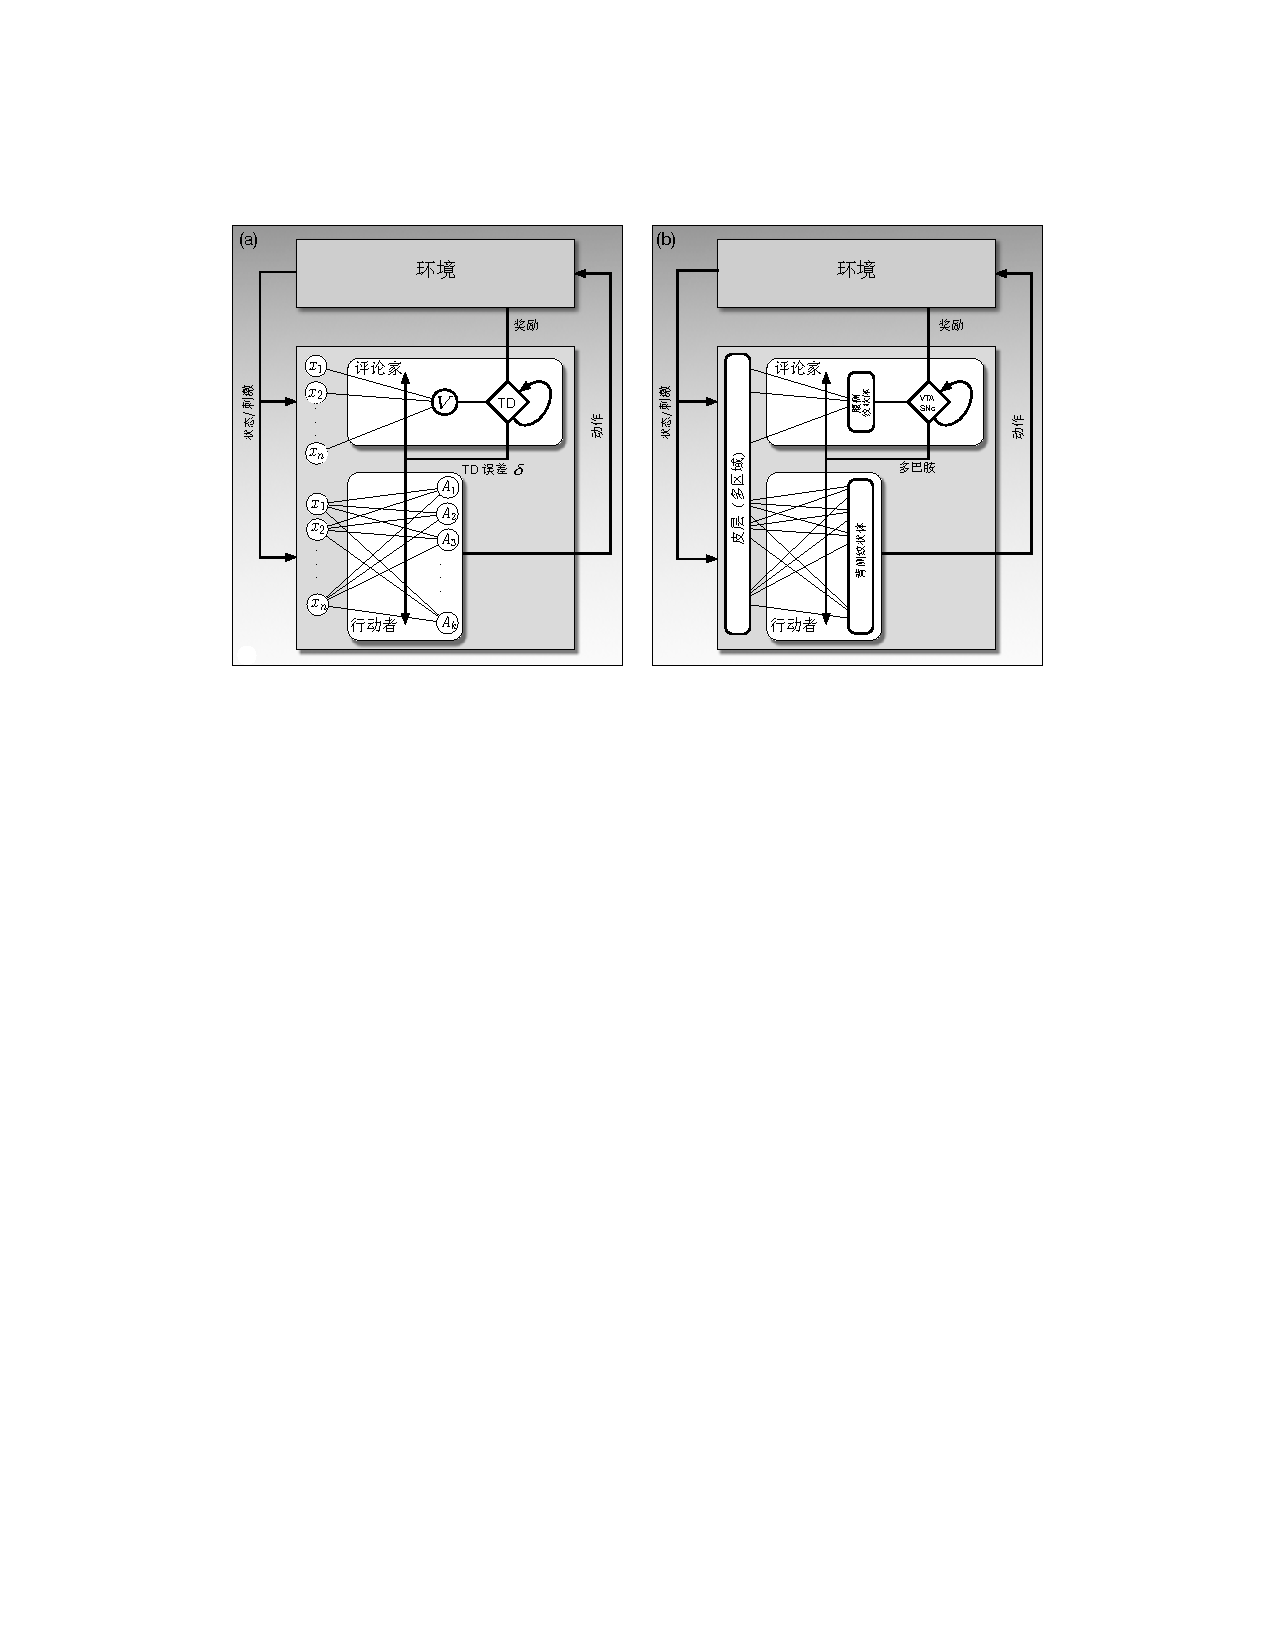
\includegraphics[width=0.8\linewidth]{chap12/fig_12_6}
	\caption{\textit{行动者-评论家}人工神经网络和假设的神经实现。
		a) 作为人工神经网络的\textit{行动者-评论家}算法。
			\textit{行动者}根据从\textit{评论家}处收到的\textit{时间差分}误差来调整策略;
			\textit{评论家}使用相同的方法调整状态值参数。
			\textit{评论家}根据奖励信号 $R$ 及其状态值估计的当前变化产生\textit{时间差分}误差。
			\textit{行动者}无法直接访问奖励信号,\textit{评论家}也无法直接访问\textit{动作}。
			b) 假设的\textit{行动者-评论家}算法的神经实现。
			\textit{评论家}和\textit{行动者}的价值学习部分分别位于腹侧纹状体和背侧纹状体。
			\textit{时间差分}误差由位于\textit{中脑腹侧被盖区}和\textit{黑质致密部}的多巴胺神经元传递,以调节从皮层区域到腹侧纹状体和背侧纹状体的输入突触效率的变化\cite{takahashi2008silencing}。
		\label{fig:12_6}}
\end{figure}


评论家和行动者网络都接收由代表智能体环境状态的多个特征组成的输入。
(回想一下第一章,强化学习智能体的环境包括包含该智能体的“有机体”内部和外部的组件。)
该图将这些特征显示为 $x_1,x_2,...,x_n$ 标记的圆圈,显示两次只是为了使图形简单。
代表突触效率的权重与从每个特征 $x_i$ 到评价单元 $V$ 以及到每个动作单元 $A_i$ 的每个连接相关联。
\textit{评论家}网络中的权重参数化\textit{价值函数},而\textit{行动者}网络中的权重参数化\textit{策略}。
当这些权重根据我们在下一节中描述的\textit{评论家}和行动者学习规则变化时,网络会进行学习。


\textit{评论家}中的回路产生的\textit{时间差分}误差是用于改变\textit{评论家}和\textit{行动者}网络中权重的增强信号。
这在图~\ref{fig:12_6}a 中通过标记为“TD error”的线显示,该线延伸到评论家和行动者网络中的所有连接。
网络实现的这一方面,加上奖励预测误差假设以及多巴胺神经元的活动通过这些神经元的广泛轴突乔木广泛分布的事实,表明像这样的\textit{行动者-评论家}网络可能不太适合 作为关于奖励相关学习如何在大脑中发生的假设是牵强的。


图~\ref{fig:12_6}b 非常示意性地表明了图左侧的人工神经网络如何根据\textit{高桥}等人的假设映射到大脑中的结构\cite{takahashi2008silencing}。
该假设将行动者和\textit{评论家}的价值学习部分分别置于纹状体的背侧和腹侧细分中,纹状体是基底神经节的输入结构。
回想一下~\ref{sec:dopamine}~节,背侧纹状体主要参与影响动作选择,而腹侧纹状体被认为对于奖励处理的不同方面至关重要,包括将情感价值分配给感觉。
大脑皮层与其他结构一起向纹状体发送输入,传达有关刺激、内部状态和运动活动的信息。


在这个假设的行动者-\textit{评论家}大脑实现中,腹侧纹状体将价值信息发送到\textit{中脑腹侧被盖区}和\textit{黑质致密部},其中这些核中的多巴胺神经元将其与奖励信息结合起来,以生成与\textit{时间差分}误差相对应的活动(尽管多巴胺能神经元究竟如何计算这些误差是还没明白)。
图~\ref{fig:12_6}~a中的“TD误差”线变成图~\ref{fig:12_6}b中标记为“多巴胺”的线,它代表多巴胺神经元的广泛分支的轴突,其细胞体位于\textit{中脑腹侧被盖区}和\textit{黑质致密部}中。
回顾图~\ref{fig:12_2},这些轴突与中型多刺神经元树突上的棘进行突触接触,中型多刺神经元是纹状体背侧和腹侧部分的主要输入/输出神经元。
将输入发送到纹状体的皮层神经元的轴突在这些棘的尖端上形成突触接触。
根据这一假设,正是在这些棘上,从皮层区域到地层的突触效率的变化受到学习规则的控制,而学习规则主要取决于多巴胺提供的强化信号。


图~\ref{fig:12_6}b 所示假设的一个重要含义是,多巴胺信号不是强化学习标量 $R_t$ 那样的“主”奖励信号。
事实上,这一假设意味着人们不一定能够探测大脑并记录任何单个神经元活动中的任何信号,如 $R_t$。
许多互连的神经系统生成与奖励相关的信息,根据不同类型的奖励而招募不同的结构。
多巴胺神经元从许多不同的大脑区域接收信息,因此图~\ref{fig:12_6}b 中标记为“奖励”的\textit{黑质致密部}和\textit{中脑腹侧被盖区}的输入应被视为沿着多个输入通道到达这些核中的神经元的奖励相关信息的向量。
那么,理论标量奖励信号 $R_t$ 可能对应的是所有奖励相关信息对多巴胺神经元活动的净贡献。
它是大脑不同区域许多神经元活动模式的结果。


尽管图~\ref{fig:12_6}b 中所示的\textit{行动者-评论家}神经实现在某些方面可能是正确的,但它显然需要细化、扩展和修改,才能成为多巴胺神经元阶段性活动功能的全面模型。
本章末尾的历史和书目评论部分引用了一些出版物,这些出版物更详细地讨论了这一假设的实证支持及其不足之处。
我们现在详细研究行动者和\textit{评论家}学习算法对控制皮层纹状体突触突触效率变化的规则的建议。





\section{行动者和评论家学习规则} \label{sec:ac_rules}

如果大脑确实实现了类似行动者-评论家算法的东西,并假设多巴胺神经元群向背侧纹状体和腹侧纹状体的皮层纹状体突触广播共同的强化信号,如图~\ref{fig:12_6}b~所示(这可能是我们上面提到的过于简单化),那么这个强化信号以不同的方式影响这两个结构的突触。
\textit{评论家}和\textit{行动者}的学习规则使用相同的强化信号,即\textit{时间差分}误差 $\delta$,但其对学习的影响对于这两个组件来说是不同的。
\textit{时间差分}误差(与\textit{资格迹}相结合)告诉行动者如何更新动作概率以达到更高价值的状态。
行动者的学习就像使用效应法则类型的学习规则的工具调节:行动者努力保持尽可能积极的态度。
另一方面,\textit{时间差分}误差(与\textit{资格迹}结合时)告诉\textit{评论家}改变价值函数参数的方向和幅度,以提高其预测准确性。
\textit{评论家}致力于使用像经典条件反射的\textit{时间差分}模型(第~\ref{sec:classical_conditioning}~节)这样的学习规则,将 $\delta$ 的幅度降低到尽可能接近于零。
\textit{评论家}和\textit{行动者}学习规则之间的差异相对简单,但这种差异对学习有深远的影响,并且对于行动者-评论家算法的工作方式至关重要。
差异仅在于每种类型的学习规则使用的\textit{资格迹}。


在像图~\ref{fig:12_6}b~所示的行动者-评论家神经网络中,可以使用多于一组的学习规则,但是,具体来说,这里我们重点关注具有\textit{资格迹}的连续问题的\textit{行动者-评论家}算法。
每次从状态 $S_t$ 转换到状态 $S_{t+1}$ 时,采取动作 $A_t$ 并接收动作 $R_{t+1}$,该算法计算时间差分误差 ($\delta$ ),然后更新\textit{资格迹}向量($z_t^w$ 和 $z_t^{\theta}$ )以及\textit{评论家}和\textit{行动者}($w$ 和 $\theta$),根据

\begin{equation}
	\delta_t = R_{t+1}
		+ \gamma \hat{v} (S_{t+1}, w)
		- \hat{v} (S_t, w),
\end{equation}


\begin{equation}
	z_t ^w = \lambda^w z_{t-1}^w
		+ \Delta_w \hat{v} (S_t, w),
\end{equation}

\begin{equation}
	z_t^{\theta} = \lambda^{\theta} z_{t-1}^{\theta}
		+ \Delta_{\theta} ln(\pi(A_t | S_t, \theta)),
\end{equation}


\begin{equation}
	w \longleftarrow w + \alpha^w \delta_t z_t^w,
\end{equation}

\begin{equation}
	\theta \longleftarrow \theta + \alpha^{\theta} \delta z_t^{\theta},
\end{equation}
其中$\gamma \in $ [0, 1) 是折扣率参数,$\lambda^w \in$ [0, 1] 和 $\lambda ^w a \in$ [0; 1] 分别是\textit{评论家}和\textit{行动者}的自举参数,$\alpha ^w$ > 0 和 $\alpha ^{\theta}$> 0 是类似的步长参数。


将近似值函数 $\hat{v}$ 视为单个线性神经元类单元的输出,称为评价单元并在图~\ref{fig:12_6}a 中标记为 $V$。
那么值函数是状态 $s$ 的特征向量表示的线性函数,$x(s) = (x_1(s), ..., x_n(s))^T$,由权重向量 $w = (w_1, ..., w_n) ^T$:

\begin{equation} \label{eq:15_1}
	\hat{v}(s, w) = w^T x(s).
\end{equation}


每个 $x_i(s)$就像神经元突触的突触前信号,其效能为 $w_i$。
\textit{评论家}的权重根据上述规则增加 $\alpha^w \delta_t z_t^w$,其中强化信号 $\delta_t$ 对应于广播到所有\textit{评论家}单元突触的多巴胺信号。
评价单位的\textit{资格迹}向量 $z_t^w$ 是 $\Delta_w \hat{v} (S_t, w)$ 的轨迹(最近值的平均值)。
因为 $\hat{v}(s, w)$ 的权重是线性的,所以 $\Delta_w \hat{v} (S_t, w) = x(S_t)$。


用神经科学术语来说,这意味着每个突触都有自己的\textit{资格迹},它是向量 $z_t^w$ 的一个组成部分。
突触的合格轨迹根据到达该突触的活动水平(即突触前活动水平)进行累积,此处由到达该突触的特征向量 $x(S_t)$ 的分量表示。
否则,迹线将以分数 $\lambda ^w$ 控制的速率向零衰减。
只要突触的\textit{资格迹}非零,它就有资格进行修改。
突触的有效性实际上如何改变取决于突触合格时到达的强化信号。
我们将像评价单元突触这样的资格痕迹称为非偶然资格痕迹,因为它们仅依赖于突触前活动,而不以任何方式取决于突触后活动。


评价单元突触的非偶然资格痕迹意味着评价单元的学习规则本质上是第~\ref{sec:classical_conditioning}~节中描述的经典条件反射的\textit{时间差分}模型。
根据我们上面给出的\textit{评论家}单元及其学习规则的定义,图~\ref{fig:12_6}a 中的\textit{评论家}与 Barto 等人的神经网络\textit{行动者-评论家}中的\textit{评论家}相同\cite{barto13neuron}。
显然,像这样仅由一个类似线性神经元的单元组成的\textit{评论家}是最简单的起点;
这个评价单元是一个更复杂的神经网络的智能体,能够学习更复杂的价值函数。


图~\ref{fig:12_6}a 中的行动者是一个由 $k$ 个类似神经元的行动者单元组成的一层网络,每个行动者在时间 $t$ 接收与\textit{评论家}单元接收的相同特征向量 $x(S_t)$。
每个行动者单元 $j, j=1, ..., k$ 有自己的权重向量 $\theta_j$ ,但由于行动者单元都是相同的,因此我们仅描述其中一个单元并省略下标。
这些单元遵循上面等式中给出的\textit{行动者-评论家}算法的一种方法是每个单元都是伯努利逻辑单元。
这意味着每个行动单元每次的输出是一个随机变量$A_t$,取值0或1。
将值1视为神经元环,即发出动作电位。
单元输入向量的加权和 $\theta^T x(S_t)$ 通过指数 softmax 分布确定单元的动作概率,对于两个动作来说,它是逻辑函数:

\begin{equation} \label{eq:15_2}
	\pi (1|s, \theta) = 
		1 - \pi(0|s, \theta) 
		= 1 \frac{1}{1 + e^{-\theta^T x(s)}}.
\end{equation}


如上所述,每个行动者单元的权重增加:$\theta \longleftarrow \theta + \alpha^{\theta} \delta_t z_t^{\theta}$,其中 $\delta$ 再次对应于多巴胺信号:发送到所有评价单元突触的相同强化信号。
图~\ref{fig:12_6}a 显示 $\delta_t$ 被广播到所有\textit{行动者}单元的所有突触(这使得该\textit{行动者}网络成为一个强化学习智能体团队,我们将在下面的~\ref{sec:collective_rl}~节中讨论)。
行动者\textit{资格迹}向量 $z_t^{\theta}$ 是 $\Delta_\theta ln \pi (A_t|S_t, \theta)$ 的轨迹(最近值的平均值)。
要了解此\textit{资格迹},它定义了此类单元并要求您为其提供学习规则。
该练习要求您通过计算梯度,用 $a$, $x(s)$ 和 $\pi(a|s, \theta)$(对于任意状态 $s$ 和动作 $a$)来表达 $\Delta _\theta ln \pi (a|s, \theta)$。
对于在时间 $t$ 实际发生的动作和状态,答案是:

\begin{equation} \label{eq:15_3}
	\nabla_{\theta} \pi (A_t | S_t, \theta)
		= (A_t - \pi(A_t|S_t, \theta)) x(S_t).
\end{equation}


与仅累积突触前活动 $x(S_t)$ 的\textit{评论家}突触的非偶然\textit{资格迹}不同,行动者单元突触的\textit{资格迹}还取决于行动者单元本身的活动。
我们称其为偶然资格痕迹,因为它取决于突触后活动。
每个突触处的合格迹线不断衰减,但增加或减少取决于突触前神经元的活动以及突触后神经元是否有反应。
当 $A_t = 1$ 时,(\ref{eq:15_3}) 中的因子 $A_t - \pi(A_t|S_t, \theta)$ 为正,否则为负。
行动者单元的资格痕迹中的突触后偶然性是\textit{评论家}和行动者学习规则之间的唯一区别。
通过保留有关在哪些州采取了哪些行动的信息,或有\textit{资格迹}允许奖励信用(正)或惩罚责备(负),以便在政策参数(行动者单位的有效性)之间进行分配。突触)根据这些参数对单元输出的贡献可能会影响以后的值。
偶然资格痕迹标记了突触,告诉它们应该如何修改以改变单元的未来反应以支持 的正值。


关于皮层纹状体突触的效率如何变化,\textit{评论家}和行动者学习规则表明了什么?
这两种学习规则都与 Donald Hebb 的经典提议相关,即每当突触前信号参与激活突触后神经元时,突触的效率就会增加\cite{hebb2005organization}。
\textit{评论家}和\textit{行动者}学习规则与赫布的提议一致,即突触效率的变化取决于多个因素的相互作用。
在评价学习规则中,相互作用发生在强化信号和仅依赖于突触前信号的\textit{资格迹}之间。
神经科学家将此称为双因素学习规则,因为相互作用是在两个信号或数量之间进行的。
另一方面,\textit{行动者}学习规则是一个三因素学习规则,因为除了取决于 $\delta$ 之外,其\textit{资格迹}还取决于突触前和突触后活动。
然而,与赫布的提议不同的是,这些因素的相对时间对于突触功效如何变化至关重要,其中资格痕迹进行干预,以允许强化信号影响最近活跃的突触。


\textit{行动者}和评论家学习规则的信号时序的一些微妙之处值得密切关注。
在定义类似神经元的\textit{行动者}和\textit{评论家}单元时,我们忽略了突触输入影响真实神经元环所需的少量时间。
当突触前神经元的动作电位到达突触时,神经递质分子被释放,穿过突触间隙到达突触后神经元,在那里它们与突触后神经元表面的受体结合;
这会激活分子机制,导致突触后神经元重新激活(或在抑制性突触输入的情况下抑制其环)。
这个过程可能需要几十毫秒。
然而,根据(\ref{eq:15_1})和(\ref{eq:15_2}),评论家和\textit{行动者}单元的输入立即产生该单元的输出。
像这样忽略激活时间在赫布式可塑性的抽象模型中很常见,其中突触效能根据同时突触前和突触后活动的简单产物而变化。
更现实的模型必须考虑激活时间。


激活时间对于更现实的\textit{行动者}单元尤其重要,因为它影响偶然资格痕迹必须如何工作,以便正确地将强化的功劳分配给适当的突触。
定义上面给出的执行者单元学习规则的条件资格迹的表达式 $(A_t - \pi(A_t|S_t, \theta)) x(S_t)$ 包括突触后因子 $(A_t, \pi(A_t | S_t, \theta))$ 和突触前因子 $x(S_t)$。
这是有效的,因为通过忽略激活时间,突触前活动 $x(S_t)$ 参与引起出现在 $(A_t - \pi(A_t | S_t, \theta))$ 中的突触后活动。
为了正确分配强化的信用,定义\textit{资格迹}的突触前因素必须是也定义轨迹的突触后因素的原因。
更现实的\textit{行动者}单位的偶然\textit{资格迹}必须考虑激活时间。
(激活时间不应与神经元接收受该神经元活动影响的强化信号所需的时间混淆。资格迹线的功能是跨越这个时间间隔,该时间间隔通常比激活时间长得多。
我们讨论这个下一节将进一步介绍。)


神经科学提供了关于这一过程如何在大脑中发挥作用的线索。
神经科学家发现了一种称为\textit{脉冲时序的可塑性}的赫布可塑性形式,它为大脑中类似\textit{行动者}的突触可塑性的存在提供了合理性。
\textit{脉冲时序的可塑性}是赫布式的可塑性,但突触功效的变化取决于突触前和突触后动作电位的相对时间。
这种依赖性可以采取不同的形式,但在研究最多的一种形式中,如果通过突触传入的尖峰在突触后神经元恢复之前不久到达,突触的强度就会增加。
如果时间关系相反,突触前尖峰在突触后神经元释放后不久到达,则突触的强度会降低。
\textit{脉冲时序的可塑性}是赫布可塑性的一种,它考虑了神经元的激活时间,这是类\textit{行动者}学习所需的要素之一。


\textit{脉冲时序的可塑性}的发现促使神经科学家研究\textit{脉冲时序的可塑性}三因素形式的可能性,其中神经调节输入必须遵循适当定时的突触前和突触后峰值。
这种形式的突触可塑性,称为奖励调节\textit{脉冲时序的可塑性},很像这里讨论的\textit{行动者}学习规则。
只有在突触前尖峰紧随其后的突触后尖峰之后的时间窗口内存在神经调节输入时,常规\textit{脉冲时序的可塑性}才会产生突触变化。
越来越多的证据表明,奖励调节的\textit{脉冲时序的可塑性}发生在背侧纹状体的中型多棘神经元的棘上,多巴胺提供了神经调节因子|在图~\ref{fig:12_6}~所示的\textit{行动者-评论家}算法的假设神经实现中,\textit{行动者}学习发生在这些位点。
b. 实验已经证明了奖赏调节\textit{脉冲时序的可塑性},其中只有当神经调节脉冲在突触前尖峰紧随其后紧随突触后尖峰之后持续长达 10 秒的时间窗口内到达时,皮层纹状体突触效能才会发生持久变化\cite{yagishita2014critical}。
尽管证据是间接的,但这些实验表明存在具有较长时间进程的偶然资格痕迹。
产生这些痕迹的分子机制,以及可能构成\textit{脉冲时序的可塑性}的更短痕迹,尚不清楚,但针对时间依赖性和神经调节剂依赖性突触可塑性的研究仍在继续。


我们在这里描述的类似神经元的行动者单元,及其效应法则式的学习规则,以某种更简单的形式出现在 Barto 等人的行动者-评论家网络中\cite{barto13neuron}。
该网络的灵感来自于生理学家\textit{克洛普夫}提出的“享乐神经元”假说\cite{klopf1972brain,klopf1982hedonistic}。
\textit{克洛普夫}假说的所有细节并不都与突触可塑性的知识相一致,但\textit{脉冲时序的可塑性}的发现以及越来越多的证据表明\textit{脉冲时序的可塑性}的奖励调节形式表明\textit{克洛普夫}的想法可能并没有离题。
接下来我们讨论\textit{克洛普夫}的享乐主义神经元假说。



\section{享乐主义神经元}


\textit{克洛普夫}\cite{klopf1972brain,klopf1982hedonistic}在他的享乐主义神经元假说中猜测,个体神经元试图通过根据自身动作电位的奖励或惩罚结果调整突触的大小,最大限度地扩大被视为奖励的突触输入和被视为惩罚的突触输入之间的差异。
换句话说,单个神经元可以通过响应相关强化进行训练,就像动物可以在工具调节任务中进行训练一样。
他的假设包括这样的想法:奖励和惩罚是通过刺激或抑制神经元尖峰生成活动的相同突触输入传递给神经元的。
(如果\textit{克洛普夫}知道我们今天对神经调节系统的了解,他可能会将强化作用分配给神经调节输入,但他想避免任何集中的训练信息来源。)
过去突触前和突触后活动的突触局部痕迹在\textit{克洛普夫}的假说中起着关键作用,即使突触有资格通过后来的奖励或惩罚进行调整。
他推测这些痕迹是由每个突触局部的分子机制实现的,因此与突触前和突触后神经元的电活动不同。
在本章的参考文献和历史评论部分,我们提请注意其他人提出的一些类似建议。


\textit{克洛普夫}具体推测突触效能以下列方式变化。
当神经元释放动作电位时,其所有积极贡献该动作电位的突触都有资格经历其功效的变化。
如果在适当的时间段内随着动作电位的增加奖励的增加,所有符合条件的突触的效率都会增加。
对称地,如果动作电位在适当的时间段内增加惩罚,则符合条件的突触的效率就会降低。
这是通过在突触那里触发资格迹来实现的,这种触发只在突触前与突触后的活动碰巧一致的时候才会发生(或者更准确地说,是在突触前活动和该突触前活动所参与引发的突触后活动同时出现的时候才会发生)。
这本质上是上一节中描述的行动者单元的三因素学习规则。


\textit{克洛普夫}理论中\textit{资格迹}的形状和时间过程反映了神经元嵌入其中的许多反馈回路的持续时间,其中一些完全位于生物体的大脑和身体内,而另一些则通过运动与感知系统延伸到机体外部的环境中。
他的想法是,突触\textit{资格迹}的形状就像神经元嵌入的反馈循环持续时间的直方图。
然后,\textit{资格迹}的峰值将出现在该神经元参与的最普遍反馈循环的持续时间内。
本书中描述的算法使用的资格迹是\textit{克洛普夫}原始想法的简化版本,是由参数 $\lambda$ 和 $\gamma$ 控制的指数(或几何)递减函数。
这简化了模拟和理论,但我们将这些简单的\textit{资格迹}视为更接近\textit{克洛普夫}原始概念的轨迹的占位符,通过改进学分分配过程,这将在复杂的强化学习系统中具有计算优势。


\textit{克洛普夫}的享乐主义神经元假说并不像乍看起来那样难以置信。
大肠杆菌是一个经过充分研究的单细胞寻求某些刺激并避免其他刺激的例子。
这种单细胞生物的运动受到其环境中化学刺激的影响,这种行为称为趋化性。
它通过旋转附着在其表面的称为 Agella 的毛发状结构,在液体环境中游泳。 (是的,它旋转它们!)细菌环境中的分子与其表面的受体结合。
结合事件调节细菌逆转无细胞旋转的频率。
每次逆转都会导致细菌原地翻滚,然后随机转向新的方向。
当细菌游向其生存所需的较高浓度的分子(引诱剂)时,少量的化学记忆和计算会导致无糖反转的频率降低,而当细菌游向有害的较高浓度的分子(排斥剂)时,无胶反转的频率会增加。
结果是,细菌倾向于持续沿着引诱剂梯度游动,并且倾向于避免沿着排斥剂梯度游动。


刚才描述的趋化行为称为调转运动。
这是一种试错行为,尽管不太可能涉及学习:细菌需要一点短期记忆来检测分子浓度梯度,但它可能无法维持长期记忆。
人工智能先驱\textit{奥利弗$\cdot$塞尔弗里奇}将这种策略称为“奔跑和旋转”,并指出其作为基本自适应策略的实用性:“如果情况变得更好,则继续以同样的方式前进,否则就四处走动”\cite{selfridge1978tracking,selfridge1984some}。
类似地,人们可能会认为神经元在由复杂的反馈回路集合组成的介质中“游泳”(当然不是字面上的意思),神经元嵌入其中,作用是获取一种类型的输入信号并避免其他类型的输入信号。
然而,与细菌不同,神经元的突触强度保留了有关其过去的试错行为的信息,如果神经元(或只是一种类型的神经元)的行为的这种观点是合理的,那么神经元如何相互作用的闭环性质。
与其环境的关系对于理解其行为非常重要,神经元的环境由动物的其余部分以及动物作为一个整体相互作用的环境组成。


\textit{克洛普夫}的享乐主义神经元假说超越了单个神经元是强化学习智能体的想法。
他认为,智能行为的许多方面可以被理解为一群自私的享乐主义神经元在构成动物神经系统的巨大社会或经济系统中相互作用的集体行为的结果。
无论这种神经系统观点是否有用,强化学习智能体的集体行为对神经科学都有影响。
我们接下来讨论这个话题。


\section{集体强化学习} \label{sec:collective_rl}

强化学习智能体群体的行为与社会和经济系统的研究密切相关,如果\textit{克洛普夫}的享乐神经元假说是正确的,那么它也与神经科学密切相关。
上面描述的关于如何在大脑中实现\textit{行动者-评论家}算法的假设仅狭隘地解决了纹状体的背侧和腹侧细分、\textit{行动者}和评论家根据假设的各自位置这一事实的含义,每个包含数百万个中型多棘神经元,其突触经历由多巴胺神经元活动的阶段性爆发调节的变化。


图~\ref{fig:12_6}a 中的\textit{行动者}是一个由 $k$ 个\textit{行动者}单元组成的单层网络。
该网络产生的行为是向量 $(A_1, A_2, ..., A_k) ^T$,被认为驱动动物的行为。
所有这些单元的突触功效的变化取决于强化信号。
因为行动者单位试图尽可能大,所以有效地充当了他们的奖励信号(因此在这种情况下,强化与奖励相同)。
因此,每个参与者单元本身就是一个强化学习主体——如果你愿意的话,就是一个享乐神经元。
现在,为了使情况尽可能简单,假设这些单元中的每个单元在同一时间接收相同的奖励信号(尽管如上所述,假设多巴胺在相同条件下在相同时间在所有皮质纹状体突触释放可能过于简单)。


当强化学习智能体群体的所有成员根据共同的奖励信号进行学习时,强化学习理论可以告诉我们什么?
多智能体强化学习领域考虑了强化学习智能体群体学习的许多方面。
尽管这个领域超出了本书的范围,但我们相信它的一些基本概念和结果与思考大脑的多功能神经调节系统相关。
在多智能体强化学习(以及博弈论)中,所有智能体试图最大化它们同时接收的公共奖励信号的场景被称为合作博弈或团队问题。


团队问题之所以有趣且具有挑战性,是因为发送给每个智能体的共同奖励信号评估了整个群体产生的活动模式,即评估了团队成员的集体行动。
这意味着任何单个智能体影响奖励信号的能力都有限,因为任何单个智能体仅贡献由公共奖励信号评估的集体行动的一个组成部分。
在这种情况下,有效的学习需要解决结构性的信用分配问题:哪些团队成员或团队成员群体应该因有利的奖励信号而受到赞扬,或因不利的奖励信号而受到指责?
这是一个合作博弈,或者说是一个团队问题,因为智能体人团结起来寻求增加相同的奖励信号:智能体之间不存在利益冲突。
如果不同的智能体收到不同的奖励信号,则该场景将是一场竞争性游戏,其中每个奖励信号再次评估群体的集体行动,并且每个智能体的目标是增加自己的奖励信号。
在这种情况下,智能体之间可能存在利益冲突,这意味着对某些智能体有利的行为对其他人不利。
甚至决定什么是最好的集体行动也是博弈论的一个重要方面。
这种竞争环境也可能与神经科学相关(例如,解释多巴胺神经元活动的异质性),但在这里我们只关注合作或团队案例。


团队中的每个强化学习智能体如何才能学会“做正确的事”,从而使团队的集体行动获得高额回报?
一个有趣的结果是,如果每个智能体都能有效地学习,尽管其奖励信号被大量破坏 尽管无法获得完整的状态信息,但总体而言,即使每个智能体无法相互沟通,总体上也会产生集体行动,这些行动会根据共同奖励信号的评估而得到改善。
它自己的强化学习任务,其中它对奖励信号的影响深深地埋藏在其他智能体的影响所产生的噪声中。
事实上,对于任何智能体来说,所有其他智能体都是其环境的一部分,因为它的输入都是其环境的一部分。
传达状态信息的部分和奖励部分取决于所有其他智能体的行为方式。
此外,由于无法访问其他智能体的操作,实际上也无法访问确定其策略的参数,因此每个智能体只能部分地观察状态。其环境。
这使得每个团队成员的学习任务非常困难,但如果每个团队成员都使用强化学习算法,即使在这些困难的条件下也能够增加奖励信号,那么强化学习智能体团队就可以学会产生随着时间的推移而改进的集体行动,如下所示: 通过团队的共同奖励信号进行评估。


如果团队成员是类似神经元的单元,那么每个单元都必须有随着时间的推移增加其收到的奖励量的目标,就像我们在第~\ref{sec:ac_rules}~节中描述的\textit{行动者}单元所做的那样。
每个单元的学习算法必须具有两个基本特征。
首先,它必须使用或有资格痕迹。
回想一下,用神经术语来说,当突触前输入参与导致突触后神经元重新激活时,突触处就会启动(或增加)偶然\textit{资格迹}。
相反,非偶然\textit{资格迹}是由突触前输入启动或增加的,与突触后神经元的行为无关。
正如第~\ref{sec:ac_rules}~节中所解释的,通过保留有关在哪些州采取了哪些行动的信息,或有\textit{资格迹}允许根据这些参数的值在哪些状态中做出的贡献,将奖励信用或惩罚责备分配给智能体的策略参数。
决定智能体的行动。
通过类似的推理,团队成员必须记住其最近的操作,以便可以根据随后收到的奖励信号增加或减少产生该操作的可能性。
或有\textit{资格迹}的操作组件实现此操作内存。
然而,由于学习任务的复杂性,偶然资格只是学分分配过程中的初步步骤:单个团队成员的行动与团队奖励信号变化之间的关系是一种统计相关性,必须在许多方面进行估计。
试验。
或有资格是这一过程中的一个重要但初步的步骤。


使用非偶然\textit{资格迹}进行学习在团队环境中根本不起作用,因为它无法提供将行为与奖励信号的后续变化相关联的方法。
非偶然\textit{资格迹}对于学习预测来说是足够的,就像行动者-\textit{评论家}算法的\textit{评论家}组件一样,但它们不支持学习控制,而行动者组件必须这样做。
类似\textit{评论家}的智能体群体的成员可能仍然会收到共同的强化信号,但他们都会学习预测相同的数量(在行动者-评论家方法的情况下,这将是当前策略的预期回报) 。
每个群体成员在学习预测预期回报方面的成功程度将取决于其收到的信息,而对于不同的群体成员来说,这些信息可能非常不同。
人们不需要产生差异化的活动模式。
这不是此处定义的团队问题。


团队问题中集体学习的第二个要求是,团队成员的行动必须具有可变性,以便团队探索集体行动的空间。
强化学习智能体团队做到这一点的最简单方法是每个成员通过其输出的持续变化独立探索自己的行动空间。
这将导致团队作为一个整体改变其集体行动。
例如,第~\ref{sec:ac_rules}~节中描述的行动者单元团队探索集体行动的空间,因为每个单元的输出(作为伯努利逻辑单元)在概率上取决于其输入向量分量的加权和。
加权和使概率出现上下偏差,但总是存在可变性。
因为每个单元都使用强化策略梯度算法(第~\ref{chap:chap11}~章),所以每个单元都会调整其权重,以最大化其经历的平均奖励率,同时随机探索自己的动作空间。
正如\textit{威廉姆斯}\cite{williams1992simple}所做的那样,我们可以证明,一组伯努利逻辑强化单元根据团队共同奖励信号的平均率整体实施了一种策略梯度算法,其中的行动是团队的集体行动 。


此外,\textit{威廉姆斯}\cite{williams1992simple}表明,当团队中的单元互连形成多层神经网络时,使用 REINFORCE 的伯努利逻辑单元团队会提升平均奖励梯度。
在这种情况下,奖励信号被广播到网络中的所有单元,尽管奖励可能仅取决于网络输出单元的集体行动。
这意味着伯努利逻辑强化单元的多层团队像通过广泛使用的误差反向传播方法训练的多层网络一样学习,但在这种情况下,反向传播过程被广播的奖励信号取代。
在实践中,误差反向传播方法要快得多,但强化学习团队方法作为一种神经机制更合理,特别是考虑到我们正在了解第~\ref{sec:ac_rules}~节中讨论的奖励调制\textit{脉冲时序的可塑性}。


团队成员自主探索只是团队探索最简单的方式;
如果团队成员能够相互沟通,以便他们能够协调行动,专注于集体行动空间的特定部分,那么更复杂的方法是可能的。
还有比偶然\textit{资格迹}更复杂的机制来解决结构性信用分配,当可能的集体行动集以某种方式受到限制时,这在团队问题中更容易。
一个极端的例子是赢者通吃的安排(例如,大脑横向抑制的结果),它将集体行动限制为只有一个或少数团队成员做出贡献的行动。
在这种情况下,获胜者会因由此产生的奖励或惩罚而受到赞扬或指责。


合作游戏(或团队问题)和非合作游戏问题的学习细节超出了本书的范围。
本章末尾的参考文献和历史评论部分引用了相关出版物的精选内容,包括对集体强化学习对神经科学的影响的研究的广泛参考。


\section{大脑中基于模型的方法}

事实证明,强化学习在无模型算法和基于模型算法之间的区别对于思考动物学习和决策过程非常有用。
第~\ref{sec:habitual_behavior}~节讨论了这种区别如何与习惯性和目标导向的动物行为之间的区别相一致。
上面讨论的关于大脑如何实现行动者/\textit{评论家}算法的假设仅与动物的习惯行为模式相关,因为基本的行动者/\textit{评论家}方法是无模型的。
哪些神经机制负责产生目标导向的行为,它们如何与那些潜在的习惯行为相互作用?


研究这些行为模式所涉及的大脑结构问题的一种方法是灭活老鼠大脑的某个区域,然后观察老鼠在结果贬值实验中的行为(第~\ref{sec:habitual_behavior}~节)。
此类实验的结果表明,上述的\textit{行动者-评论家}假设将\textit{行动者}置于背侧纹状体方面过于简单。
背侧纹状体的一部分——\textit{背外侧纹状体}失活会损害习惯学习,导致动物更多地依赖目标导向的过程。
另一方面,\textit{背内侧纹状体}失活会损害目标导向过程,要求动物更多地依赖习惯学习。
这些结果支持这样的观点:啮齿类动物的\textit{背外侧纹状体}更多地参与无模型过程,而它们的\textit{背内侧纹状体}更多地参与基于模型的过程。
使用功能神经影像学对人类受试者和非人类灵长类动物进行类似实验的研究结果支持这样的观点,即灵长类动物大脑中的类似结构不同地涉及习惯性和目标导向的行为模式。


其他研究确定了与人脑前额叶皮层基于模型的过程相关的活动,额叶皮层的最前部涉及执行功能,包括计划和决策。
特别涉及的是\textit{眶额皮层},即\textit{前额叶皮层}紧邻眼睛上方的部分。
人类的功能神经成像以及猴子单个神经元活动的记录揭示了\textit{眶额皮层}中与生物显着刺激的主观奖励值相关的强烈活动,以及与行动结果预期奖励相关的活动。
虽然并非没有争议,但这些结果表明\textit{眶额皮层}在目标导向选择中发挥了重要作用。
这对于动物环境模型的奖励部分可能至关重要。


涉及基于模型的行为的另一个结构是海马体,它是记忆和空间导航的关键结构。
大鼠的海马体在大鼠以目标导向的方式穿越迷宫的能力中发挥着关键作用,这导致托尔曼得出动物在选择行动时使用模型或认知图的想法(第~\ref{sec:cognitive_maps}~节)。
海马体也可能是我们人类想象新体验能力的关键组成部分\cite{hassabis2007deconstructing,olafsdottir2015hippocampal}。


最直接地将海马体与计划联系在一起的发现——这是一个在做出决策时寻求环境模型所需的过程——来自于对海马体中神经元的活动进行解码的实验,以确定海马体活动在每时每刻的基础上代表了哪一部分空间。
当老鼠在迷宫中的某个选择点停下来时,海马体中的空间表示会沿着动物从该点开始可能采取的路径向前(而不是向后)扫过\cite{johnson2007neural}。
此外,这些扫描所代表的空间轨迹与大鼠随后的导航行为密切对应\cite{pfeiffer2013hippocampal}。
这些结果表明,海马体对动物环境模型的状态转换部分至关重要,它是一个系统的一部分,该系统使用该模型模拟未来可能的状态序列,以评估可能的行动过程的后果:一种规划形式。


上述结果丰富了有关目标导向或基于模型的学习和决策的神经机制的大量文献,但许多问题仍未得到解答。
例如,像\textit{背外侧纹状体}和\textit{背内侧纹状体}这样结构相似的领域如何成为像无模型算法和基于模型算法一样不同的学习和行为模式的重要组成部分?
单独的结构是否负责(我们所说的)环境模型的转换和奖励组件?
所有计划是否都是在决策时通过模拟未来可能的行动方案来进行的,正如海马体中的前向扫荡活动所暗示的那样?
换句话说,所有的计划都类似于推出算法(第~\ref{sec:collective_rl}~节)吗?
或者模型有时会在后台进行细化或重新计算价值信息,如 Dyna 架构(第~\ref{sec:reward_signals}~节)所示?
大脑如何在习惯和目标导向系统的使用之间进行仲裁?
事实上,这些系统的神经基质之间是否存在明显的分离?


证据并未对最后一个问题给出肯定的答案。
Doll\cite{doll2012ubiquity}总结了这种情况,写道“在大脑处理奖励信息的任何地方,基于模型的影响或多或少都无处不在”,即使在被认为对无模型至关重要的区域也是如此。
这包括多巴胺信号本身,除了被认为是无模型过程基础的奖励预测误差之外,它还可以表现出基于模型的信息的影响。


以强化学习的无模型和基于模型的区别为基础的持续神经科学研究有可能加深我们对大脑中习惯性和目标导向过程的理解。
更好地掌握这些神经机制可能会导致算法以计算强化学习中尚未探索的方式结合无模型和基于模型的方法。


\section{成瘾}


了解药物滥用的神经基础是神经科学的一个高度优先目标,有可能为这一严重的公共卫生问题产生新的治疗方法。
一种观点认为,对毒品的渴望是同样的动机和学习过程的结果,这些动机和学习过程引导我们寻求满足我们生物需求的自然奖励体验。
成瘾物质通过强烈强化,有效地吸收了我们学习和决策的自然机制。
这是合理的,因为许多(尽管不是全部)滥用药物直接或间接增加了纹状体中多巴胺神经元轴突末端周围区域的多巴胺水平,纹状体是一种与正常奖励学习密切相关的大脑结构(第~\ref{sec:neural_ac}~节)。
但与毒瘾相关的自我毁灭行为并不是正常学习的特征。
当奖励是成瘾药物的结果时,多巴胺介导的学习有何不同?
成瘾是否是对物质的正常学习的结果,而这些物质在我们的进化史上基本上是不可用的,因此进化无法选择对抗它们的破坏性影响?
或者成瘾物质是否会以某种方式干扰正常的多巴胺介导的学习?


多巴胺神经元活动的奖励预测误差假设及其与\textit{时间差分}学习的联系是 Redish\cite{redish2004addiction} 的模型的基础,该模型描述了成瘾的一些(但肯定不是全部)特征。
该模型基于这样的观察:服用可卡因和其他一些成瘾药物会导致多巴胺短暂增加。
在模型中,假设这种多巴胺激增会增加\textit{时间差分}误差 ,其方式无法通过价值函数的变化来抵消。
换句话说,虽然减少到正常奖励由先行事件预测的程度(第~\ref{sec:td_dopamine}~节),但成瘾刺激的贡献不会随着奖励信号的预测而减少:药物奖励不能被预测。
该模型通过防止奖励信号因成瘾药物而变为负值来实现这一点,从而消除了与药物管理相关的状态的\textit{时间差分}学习的纠错功能。
结果是,值 这些状态的数量无限增加,使得导致这些状态的行动优先于所有其他状态。


成瘾行为比雷迪什模型的结果要复杂得多,但该模型的主要思想可能只是谜题的一部分。
或者模型可能会产生误导。
多巴胺似乎并未在所有形式的成瘾中发挥关键作用,而且并非每个人都同样容易出现成瘾行为。
此外,该模型不包括伴随长期吸毒而发生的许多回路和大脑区域的变化,例如,重复使用导致药物效果减弱的变化。
成瘾也可能涉及基于模型的过程。
尽管如此,雷迪什的模型仍然说明了如何利用强化学习理论来理解重大健康问题。
以类似的方式,强化学习理论对计算精神病学新领域的发展产生了影响,该领域旨在通过数学和计算方法提高对精神障碍的理解。


\section{总结}

大脑奖励系统涉及的神经通路非常复杂且尚未完全了解,但旨在了解这些通路及其在行为中作用的神经科学研究正在迅速进展。
这项研究揭示了大脑的奖励系统与本书中提出的强化学习理论之间惊人的对应关系。


多巴胺神经元活动的奖励预测误差假说是由科学家提出的,他们认识到\textit{时间差分误差}的行为与产生多巴胺的神经元活动之间存在惊人的相似之处,多巴胺是哺乳动物中与奖励相关的学习和行为所必需的神经递质。
神经科学家\textit{舒尔茨}实验室于 20 世纪 80 年代末和 90 年代进行的实验表明,只有当动物没有预料到这些事件时,多巴胺神经元才会以大量的活动爆发(称为阶段性反应)对奖励事件做出反应,这表明多巴胺神经元正在发出奖励信号预测误差而不是奖励本身。
此外,这些实验表明,当动物学会根据先前的感觉线索预测奖励事件时,多巴胺神经元的阶段性活动会转向较早的预测线索,同时减少到较晚的预测线索。
这与强化学习智能体学习预测奖励时\textit{时间差分}误差的后备效应类似。


其他实验结果有力地证实,多巴胺神经元的阶段性活动是学习的强化信号,通过产生多巴胺的神经元的大量分支轴突到达大脑的多个区域。
这些结果与我们对奖励信号 Rt 和强化信号(即我们提出的大多数算法中的\textit{时间差分}误差 t)之间的区别是一致的。
多巴胺神经元的阶段性反应是强化信号,而不是奖励信号。


一个突出的假设是,大脑实现了类似\textit{行动者}/评论家算法的东西。
大脑中的两个结构(纹状体的背侧和腹侧部分)在基于奖励的学习中都发挥着关键作用,可能分别像\textit{行动者}和\textit{评论家}一样发挥作用。
\textit{时间差分}误差对于\textit{行动者}和\textit{评论家}来说都是强化信号,这与多巴胺神经元轴突同时针对纹状体的背侧和腹侧细分这一事实相吻合;
多巴胺似乎对于调节这两种结构的突触可塑性至关重要;
并且诸如多巴胺的神经调节剂对靶结构的影响取决于靶结构的性质而不仅仅取决于神经调节剂的性质。


行动者和\textit{评论家}可以通过由类似神经元的单元组成的人工神经网络来实现,该网络具有基于第 13.5 节中描述的策略梯度行动者/\textit{评论家}方法的学习规则。
这些网络中的每个连接就像大脑中神经元之间的突触,学习规则对应于控制突触效率如何随着突触前和突触后神经元的活动而变化的规则,以及与来自神经元的输入相对应的神经调节输入。
多巴胺神经元。
在此设置中,每个突触都有自己的\textit{资格迹},记录涉及该突触的过去活动。
行动者和\textit{评论家}学习规则之间的唯一区别在于它们使用不同类型的\textit{资格迹}:\textit{评论家}单元的轨迹是非偶然的,因为它们不涉及\textit{评论家}单元的输出,而行动者单元的轨迹是偶然的,因为另外 对于执行者单元的输入,它们取决于执行者单元的输出。
在大脑中\textit{行动者}评价系统的假设实现中,这些学习规则分别对应于控制皮质纹状体突触可塑性的规则,这些突触将信号从皮质传递到背侧和腹侧纹状体细分中的主要神经元,突触还接收来自 多巴胺神经元。


\textit{行动者-评论家}网络中的行动者单元的学习规则与奖励调节的尖峰时间依赖性可塑性密切对应。
在\textit{脉冲时序的可塑性}中,突触前和突触后活动的相对时间决定了突触变化的方向。
在奖励调节\textit{脉冲时序的可塑性}中,突触的变化还取决于神经调节剂(例如多巴胺)在满足\textit{脉冲时序的可塑性}条件后可持续长达 10 秒的时间窗口内到达。
越来越多的证据表明,奖励调节的\textit{脉冲时序的可塑性}发生在皮质纹状体突触处,其中行动者的学习发生在行动者-\textit{评论家}系统的假设神经实现中,这增加了一些动物的大脑中存在类似\textit{行动者-评论家}系统的假设的合理性。


突触资格的思想和行动者学习规则的基本特征源自\textit{克洛普夫}的“享乐神经元”假设\cite{klopf1972brain,klopf1982hedonistic}。
他推测个体神经元通过调整效率来寻求获得奖励并避免惩罚。
根据其动作电位的奖励或惩罚后果来控制突触的行为,神经元的活动可以影响其后来的输入,因为神经元嵌入在许多反馈回路中,其中一些反馈回路位于动物的神经系统和身体内,另一些则通过动物的外部。
\textit{克洛普夫}关于资格的想法是,如果突触参与了神经元环,则它们会被暂时标记为有资格进行修改(使其成为\textit{资格迹}的偶然形式),如果增强信号到达,突触的有效性就会被修改。
我们以细菌的趋化行为作为单细胞指导其运动以寻找某些分子并避开其他分子的例子。


多巴胺系统的一个显着特征是释放多巴胺的纤维广泛投射到大脑的多个部位。
尽管很可能只有某些多巴胺神经元群体广播相同的强化信号,但如果该信号到达参与\textit{行动者}型学习的许多神经元的突触,那么这种情况可以建模为团队问题。
在此类问题中,强化学习智能体集合中的每个智能体都会收到相同的强化信号,其中该信号取决于该集合或团队的所有成员的活动。
如果每个团队成员都使用足够强大的学习算法,即使团队成员彼此不直接沟通,团队也可以集体学习,以通过全球广播的强化信号评估来提高整个团队的绩效。
这与大脑中多巴胺信号的广泛分散相一致,并为广泛使用的用于训练多层网络的误差反向传播方法提供了一种神经学上合理的替代方案。


% 基于模型 -- 目标导向?
\textit{无模型}的强化学习和\textit{基于模型}的强化学习之间的区别正在帮助神经科学家研究\textit{习惯性}和\textit{目标导向}的学习和决策的神经基础。
迄今为止的研究表明,某些大脑区域比另一种过程更多地参与一种类型的过程,但情况仍不清楚,因为无模型和基于模型的过程在大脑中似乎没有被整齐地分开。
许多问题仍然没有答案。
也许最有趣的是有证据表明,海马体这种传统上与空间导航和记忆相关的结构,似乎参与\textit{模拟未来可能的行动过程},作为动物决策过程的一部分。
这表明它是使用环境模型进行规划的系统的一部分。


强化学习理论也影响着对药物滥用背后的神经过程的思考。
毒瘾某些特征的模型基于奖励预测误差假设。
它提出,可卡因等成瘾兴奋剂会破坏\textit{时间差分}学习的稳定性,从而导致与吸毒相关的行为价值无限增长。
这远不是一个完整的成瘾模型,但它说明了如何从计算角度提出可以通过进一步研究进行测试的理论。
计算精神病学的新领域同样侧重于使用计算模型(其中一些模型源自强化学习)来更好地理解精神障碍。



本章仅触及强化学习的神经科学与计算机科学与工程中的强化学习的发展如何相互影响的表面。
强化学习算法的大多数功能都将其设计归因于纯粹的计算考虑,但有些功能受到有关神经学习机制的假设的影响。
值得注意的是,随着有关大脑奖励过程的实验数据不断积累,强化学习算法的许多纯粹由计算驱动的特征被证明与神经科学数据是一致的。
计算强化学习的其他特征,例如\textit{资格迹}和强化学习智能体团队在全球广播强化信号的影响下学习集体行动的能力,也可能会变成平行的实验数据,因为神经科学家继续解开这个问题。
基于奖励的动物学习和行为的神经基础。








